% В этом файле следует писать текст работы, разбивая его на
% разделы (section), подразделы (subsection) и, если нужно,
% главы (chapter).

% Предварительно следует указать необходимую информацию
% в файле SETUP.tex

\input{preamble.tex}

\begin{document}

\Intro

При работе с электронным документооборотом остро становится проблема эффективного извлечения информации из имеющейся базы, с минимальными временными затратами. Крайне важно иметь инструмент, который бы в полуавтоматизированном режиме мог извлекать наиболее ценные с точки зрения информационного содержания отрывки из текстовых документов, избавляя пользователя от необходимости просматривать и анализировать их вручную. Поскольку нередки случаи, когда информационный объем может быть поистине огромным, ручной анализ может представлять из себя крайне затяжную и монотонную работу, отдача от которой не слишком велика.

Подобный инструмент, позволяющий с небольшой помощью со стороны пользователя извлекать действительно важную информацию из большого объема данных, оказывается крайне полезен и в других областях. Например, там, где нужно наиболее емко, но при этом достаточно кратко, описать некий товар, услугу, событие или явление. Или в системах, для которых важно предоставлять пользователю наиболее релевантные данные, важность которых оценивается на основе его предыдущих действий. Например, новостным ресурсам имеет смысл предлагать пользователю после чтения статьи обратить внимание на другие статьи с похожей тематикой.

Для того, что подобный инструмент хорошо выполнял свою работу и был удобен и прост в использовании, очень важно тщательно его спроектировать и продумать все детали его реализации. Важно разработать качественный алгоритм анализа входного текста, который будет включать в том числе этап обработки естественного языка. Не менее важно грамотно продумать взаимодействие с пользователем: язык команд, которые принимает программа, должен быть достаточно простым, но при этом поддерживать довольно широкий набор возможностей.

Открытые инструменты извлечения информации из больших объемов данных уже существуют, но они, как правило, довольно специфичны и не вполне подходят для работы со слабоструктурированными документами. Такие документы, в отличие от неструктурированного текста, имеют ряд определенных свойств, которые могут значительно повысить эффективность извлечения информации. 

Именно разработке инструмента, который бы использовал сильные стороны уже существующих решений, при этом учитывая специфику слабоструктурированных документов, посвящена данная работа.
% Если typeOfWork в SETUP.tex задан как 2 или 3, то начинать
% надо не с section (раздел), а с главы (chapter)
\chapter{Теоретические и практические подходы, применяемые для извлечения фактов из слабоструктурированных текстовых документов}
\section{Основные теоретические понятия}
\subsection{Понятие слабоструктурированного документа}
Под слабоструктурированными документами подразумеваются текстовые источники данных, которые характеризуются следующим набором признаков и свойств~\autocite{WeakStructuredDocs}:
\begin{itemize}
  \item Документ содержит в том или ином виду внутреннюю разметку.
  \item Разбиение содержимого документа на фрагменты средствами внутреннего форматирования.
  \item Фрагменты документа представляют собой информационные поля, либо же значения информационных полей.
  \item По внутренней разметке документа нельзя однозначно определить, является ли фрагмент полем, либо же значением поля.
\end{itemize}
В качестве примера слабоструктурированного документа можно взять договор. Договор как таковой характеризуется определенным набором информационных полей и их значений. Например, каждый договор должен содержать названия контрагентов, а также имена и должности физических лиц, подписывающих договор. Однако же в общем и целом два среднестатистических договора могут весьма значительно отличаться по структуре, по скольку правила оформления договоров оставляют довольно большое место для импровизации путем добавления/удаления тех или иных полей. В конечном счете нельзя однозначно сказать для заданного информационного поля, в какой части документа его искать и будет ли оно там вообще.

Также можно выделить неструктурированные документы и структурированные. Первые представляют собой текстовый документ произвольного формата. Вторые характеризуются строгим набором правил форматирования, который позволяет однозначно интерпретировать такие документы и извлекать из них информацию.

В качестве примера структурированного документа можно привести бланк квитанции на оплату коммунальных услуг на рисунке \ref{fig:ege-blank}. Данный бланк имеет строго заданную пространственную структуру документа, что позволяет довольно легко идентифицировать информационные поля.

\begin{figure}% p означает, что нужно выделить для рисунка
\centering
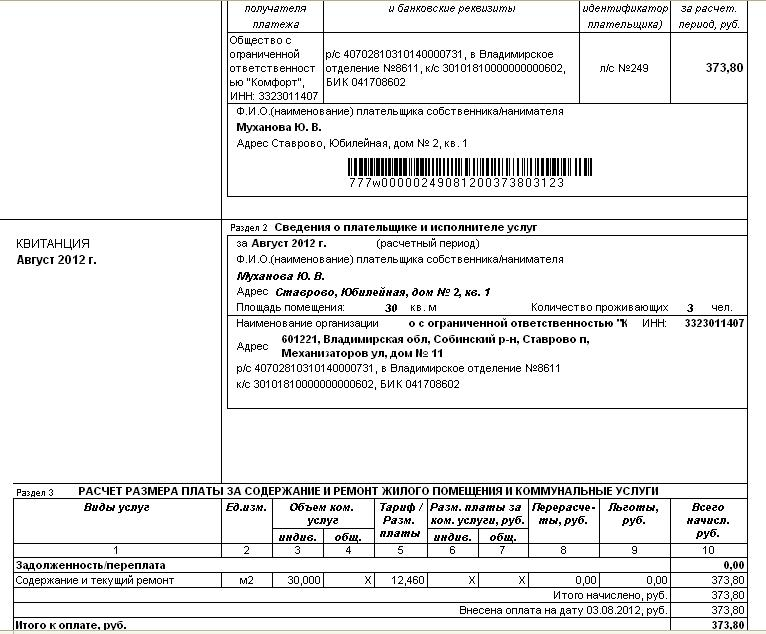
\includegraphics[width=0.7\textwidth]{img/blank.jpg}
\caption{Бланк квитанции на оплату коммунальных услуг}
\label{fig:ege-blank}
\end{figure}

\section{Извлечение информации из слабоструктурированных документов}
\subsection{Общее описание подхода}
Среди основных подходов, применяемых при извлечении информационных полей, можно выделить три основных: семантический анализ, структурный анализ и пространственный анализ.

Семантический подход предполагает анализ полноценный анализ языковых свойств текста: морфологическую разметку текста, выделение семантических и смысловых связей. При данном подходе мы пытаемся <<понять>> текст, выделить из него смысловую нагрузку, и использовать эти данные с целью как можно точнее идентифицировать нужную информацию. Среди систем, осуществляющих анализ с помощью данного подхода, можно выделить <<Томита-парсер>>~\autocite{tomita-parser}. Эта программа, разработанная в компании <<Яндекс>>, позволяет извлекать факты из произвольного текста на основе вручную заданных правил.

Структурный подход предполагает выделение из текста некоторых смысловых единиц, которые характеризуются более или менее строгой структурой (например, на разделы в случае договора, или на функции в случае программы на языке C), и затем использовать эти данные в процессе извлечения информации. В качестве примера можно привести компилятор языка C, который использует информацию о синтаксисе языка, заложенную в стандарте, для разбора программы и преобразования ее в нативный код. Если взять ту же функцию, то компилятор точно знает, как эта функция может быть записана, где ее нужно искать и где ее быть не может.

Пространственный подход предполагает, что мы более-менее точно знаем расположение различных информационных структур внутри документа: как в абсолютных выражении, так и относительно друг друга. К документам, которые поддаются подобному виду анализа, можно отнести различного вида бланки, паспорта, водительские права, квитанции и так далее.

При анализе слабоструктурированных документов важно было использовать в той или иной мере все три вышеописанных подхода, поскольку по отдельности ни один из них не в состоянии обеспечить должного качества работы.

\subsection{Концепция решения}
В качестве решения задачи было решено разработать систему извлечения информационных полей, которая:
\begin{itemize}
  \item Работала бы с широким спектром слабоструктурированных документов (для начала решено было сосредоточиться на договорах).
  \item Поддерживала бы обработку пользовательских запросов с возможность описать достаточно сложные и разнообразные виды полей. При этом язык описания должен был быть максимально простым и понятным, с привычным синтаксисом.
\end{itemize}
В результате было спроектировано решение, которое:
\begin{itemize}
  \item Принимает на вход:
  \begin{itemize}
    \item Текст договора в формате plain text.
    \item Набор правил, описывающих извлекаемые информационные поля.
  \end{itemize}
  \item Производит анализ и морфологическую разметку текста входного документа. Под морфологической разметкой подразумевается разбиение текста на элементарные единицы (слова) и выделение для каждой такой единицы присущих ей морфологических свойств. Эта часть относится к семантическому анализу, иными словами тут мы пытаемся в определенной мере <<понять>> текст.
  \item Производит компиляцию пользовательских правил в конечный автомат.
  \item Выполняет разбор входного текста (уже размеченного) с помощью конечного автомата по алгоритму Томиты.~\autocite{tomita-algorithm}
  \item Представляет пользователю результаты работы.
\end{itemize}

\subsection{Алгоритм Томиты}
Алгоритм Томиты~\autocite{tomita-algorithm} предоставляет возможность осуществлять разбор с помощью парсера, построенного на основе неоднозначной грамматики. Т.е. такой грамматики, которая содержит конфликты вида Shift/Reduce или Reduce/Reduce. Такие конфликты неизбежны, когда речь идет о естественном языке, поскольку зачастую языковые конструкции можно трактовать по-разному как с морфологической, семантической и других точек зрения.

Алгоритм Томиты или алгоритм GLR-парсинга~\autocite{tomita-algorithm} успешно справляется с такими ситуациями, позволяя разветвлять процесс разбора в случае конфликтов. Классический алгоритм LR-разбора предназначен для анализа текстов, написанных на достаточно строго детерминированных языках программирования, и с естественным языком работать не может. Томита решил эту проблему путем параллелизации стеков, что позволило рассматривать различные трактовки тех или иных участков текста: как только возникает возможность различной трактовки, стек разветвляется. Таких последовательных разветвлений может быть несколько, но в процессе анализа ошибочные ветви отбрасываются, и результатом становится наиболее длинная цепочка. При этом алгоритм выдает результаты своей работы в режиме реального времени, по мере продвижения вглубь текста, другие алгоритмы обработки естественного языка такой особенностью не обладают.

\subsection{Томита-парсер}
Томита-парсер~\autocite{tomita-parser} назван в честь японского ученого Масару Томиты, разработавшего одноименный алгоритм~\autocite{tomita-habr}. Томита-парсер применяет этот алгоритм при разборе текста на естественном языке.

В простейшем случае парсеру на входе отдается сам анализируемый текст, а также словарь и грамматика. Объем словаря и сложность грамматики зависят от целей анализа: они могут быть как совсем маленькими, так и огромными. Файл грамматики состоит из шаблонов, написанных на внутреннем языке/формализме Томита-парсера. Эти шаблоны описывают в обобщенном виде цепочки слов, которые могут встретиться в тексте. Кроме того, грамматики определяют, как именно нужно представлять извлеченные факты в итоговом выводе.

На выходе Томита-парсер выдает набор фактов, соответствующих шаблонам, описанным в файле с грамматикой.

Томита-парсер используется рядом сервисов Яндекса, включая Почта, Новости, Авто, Работа~\autocite{tomita-habr}.

\chapter{Программная реализация}
\section{Общая структура проекта}
Разработанная программа является консольным приложением, которое принимает на вход файл с текстом документа вместе с набором правил, и возвращает последовательность пар (FieldName, FieldValue), где FieldName - название информационного поля (задается в файле с правилами), а FieldValue - его значение.

Схему работы программы можно видеть на рисунке \ref{fig:project-diagram}. Программа содержит три основных модуля: 
\begin{itemize}
  \item Модуль разбора и разметки входного текста.
  \item Модуль разбора пользовательских правил.
  \item Модуль построения GLR-парсера~\autocite{tomita-algorithm}.
\end{itemize}

Первый модуль обрабатывает входной текст. Текст очищается от лишних символов и разбивается на группы токенов так, что каждая группа соответствует одному абзацу. Токены представляют собой последовательности букв и цифр, которые соответствуют словам в тексте документа. Каждый токен анализируется и соответствующим образом помечается. Например, сохраняется информация о части речи токена, и многих других морфологических характеристиках. Для разметки используется библиотека pymorphy2~\autocite{pymorphy2-home}. В конце формируется массив, содержащий упорядоченную последовательности групп токенов. Именно элементы этой последовательности затем принимает парсер.

Второй модуль обрабатывает пользовательские правила. Правила записываются в текстовый файл в строго определенном формате. Файл быть размечен на две секции: секцию описания правил и секцию команд. Первая секция предназначена для описания пользовательских правил, вторая - для указания правил, которые нужно найти. Искомое правило должно быть либо определено вручную в секции правил, либо же являться встроенным. Полученный файл с правилом затем передается на обработку программе GNU Bison~\autocite{bison-home}. Она обрабатывает файл, строит для него парсер по заранее заданной грамматике и разбирает, в процессе накапливая информацию об описанных правилах и командах.

Третий модуль непосредственно строит GLR-парсер, с помощью которого анализируется текст документа. На вход ему поступает информацию, накопленная в модуле разбора пользовательских правил. На основе полученной информации строится одна или несколько грамматик. Их количество зависит числа уникальных правил, которые помечены пользователем как цели для поиска. Затем для каждой из построенных построенных грамматик запускается процесс построения парсера, который состоит из нескольких этапов.
\begin{enumerate}
  \item Построение коллекции LR(0) пунктов.
  \item Определение множеств First Set для каждого терминала и нетерминала грамматики.
  \item Определение множеств Follow Set для каждого нетерминала грамматики, которые строятся на основе FirstSet из предыдущего пункта.
  \item Построение таблицы переходов. Набор LR(0) пунктов соответствует состояниям выстраиваемого автомата. Таким образом, для LR(0) пункта мы создаем соответствующую запись в таблице переходов.
\end{enumerate}
На основе построенной таблицы переходов реализуется алгоритм GLR-разбора. Самой главной его отличительной особенностью является то, что он способен корректно обрабатывать грамматики, содержащие конфликты типа Shift/Reduce и/или Reduce/Reduce. При обнаружении конфликтов в процессе разбора стек разветвляется и разбор продолжается уже для $N+1$ ветки.

\begin{figure}% p означает, что нужно выделить для рисунка
% отдельную страницу; применяется для больших рисунков
\centering
%Здесь могла быть ваша лягушка.
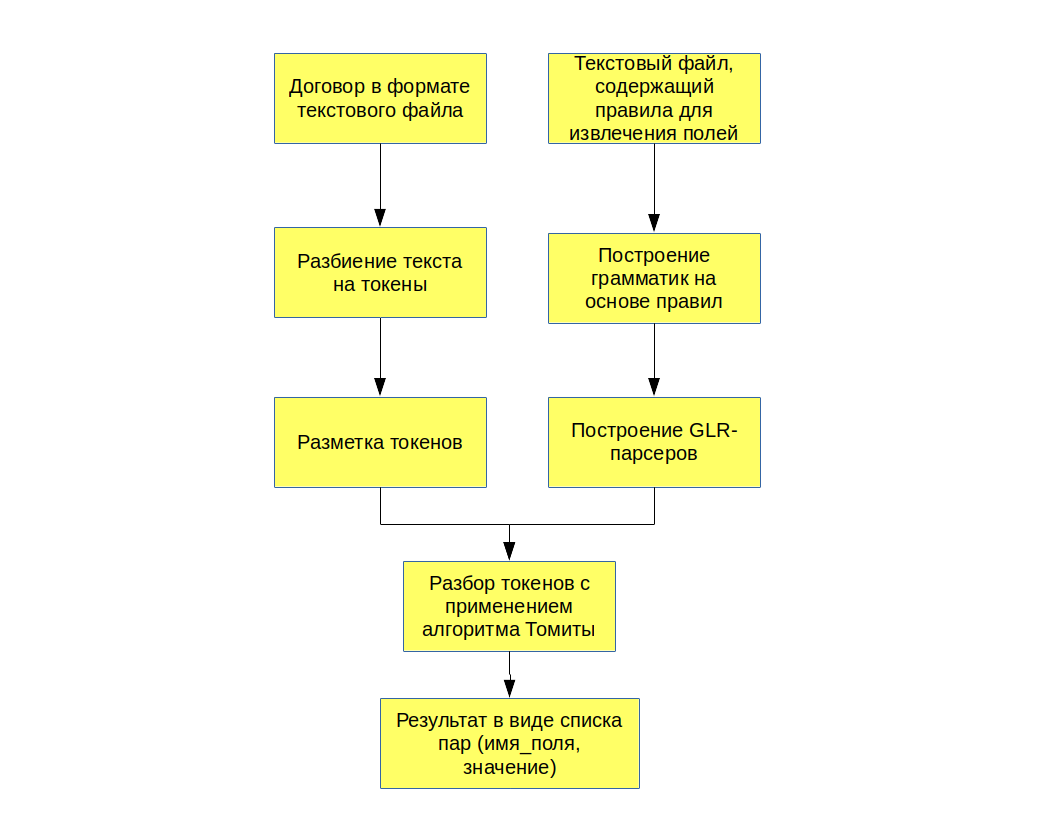
\includegraphics[width=\textwidth]{img/ProjectDiagram.png}
\caption{\label{fig:project-diagram}Схема работы программы}
\label{fig:project-diagram}
\end{figure}

\section{Разбор входного текста}
\subsection{Поддерживаемые форматы}
Документ должен поступать на вход в формате plain text. Предполагается, что файл был получен средствами офисного редактора путем экспортирования документа в формат txt. Для работы именно с такими файлами разрабатывалась и тестировалась та часть программной реализации, которая отвечает за обработку входных текстов. Любые внесенные вручную правки и коррективы могут негативно сказаться на эффективности работы программы.

Основным языком документа должен быть русский. Однако стоит отметить, что текст на других языках будет принят программой и успешно обработан. Более того, если речь идет об английском языке, можно будет даже сформировать набор правил для извлечения определенной информации из такого текста. Однако же это скорее <<побочный эффект>>, нежели самоцель. Реализация нацелена именно на работу с русским языком, и для остальных корректная работа не гарантируется. В лучшем случае будет недоступна часть функционала, в худшем - может произойти что угодно, начиная от ошибки при компиляции правил, и заканчивая аварийным завершением. Связано это главным образом с тем, что при разборе программа в немалой степени опирается на морфологические характеристики слов, и получение таких характеристик реализовано только для русского языка.

На данный момент наилучшая поддержка среди всех типов официальных документов реализована именно для договоров. Для них заготовлено несколько встроенных правил, позволяющих извлекать специфические для этого типа документов поля. Однако же поля, описывающие более общую информацию, такую как имя человека, адрес, теоретически можно извлечь из текстовых файлов произвольного формата, составленных на русском языке, как деловых, так и художественных. При составлении таких правил были учтены различные вариации написания, что позволяет заявлять высокий уровень универсальности.

Для входных файлов поддерживается только формат txt (plain text). В процессе написания программы рассматривался также ряд дополнительных форматов, для которых было бы логично обеспечить поддержку - в первую очередь, это наиболее популярные офисные форматы: DOCX, DOC, ODT. Более того, имелись идеи касательно того, что метаданные этих форматов можно было бы использовать как дополнительный источник информации, позволяющий идентифицировать поле. Например, мы знаем, что номер телефона одного из контрагентов очень часто можно найти в разделе, содержащем слово <<реквизиты>>. Тогда на основе анализа метаданных формата мы могли бы довольно легко получить список разделов, найти среди них нужный, и, получив текст для него текст, искать уже более точечно. При работе с сырым текстом для реализации чего-то подобного приходится уже прибегать к регулярным выражениям, которые предоставляют гораздо меньший уровень надежности анализа. Нет никаких гарантий того, что паттерн, описывающий заголовок раздела, не совпадет с рядовым участком текста.

Однако было решено ограничиться одним форматом, поскольку реализация поддержки форматов от Microsoft оказалась сопряжена с рядом технических трудностей вследствие объема спецификаций по формату DOCX~\autocite{Open-Office-XML} и отсутствия таковых в случае с DOC~\autocite{DOC-Format}. В итоге было решено уделить больше внимания алгоритмической части работы.

\subsection{Разбор текста на фрагменты и разметка}
Разбор и разметка входного текста производится в несколько последовательных этапов:
\begin{enumerate}
  \item Разбиение текста на абзацы по символу перехода на новую строку.
  \item Каждый абзац разбивается по определенному набору символов на последовательность слов.
  \item Для каждого слова производится морфологический анализ и нормализация.
\end{enumerate}
В конечном итоге получается массив из упорядоченных последовательностей токенов.

Сущность <<токен>> инкапсулирует слово и совокупность его характеристик.
\begin{ListingEnv}
\begin{Verb}

struct Token {
    // слово, полученное в результате разбиения абзаца
    UnicodeString word;
    // нормализованное слово
    UnicodeString normalForm;
    // часть речи
    UnicodeString partOfSpeech;
    // битовая маска, которая содержит 
    // совокупность морфологических характеристик
    unsigned propMask = 0;
    ...
};
\end{Verb}
\caption{Объявление класса Token}
\label{list:TokenClass}
\end{ListingEnv}
Как можно увидеть из листинга \ref{list:TokenClass}, \lstinline{Token} содержит битовую маску, на которую накладываются его морфологические характеристики. Эта маска формируется из перечисления \lstinline{MorphProperty}. Его объявление показано в листинге \ref{list:MorphProperty}.
\begin{ListingEnv}
\begin{Verb}

enum MorphProperty {
    // имя
    FIRST_NAME = 01,
    // фамилия
    SECOND_NAME = 02,
    // отчество
    PATR = 04,
    // инициал
    INIT = 010,
    // географический объект
    GEOX = 020,
    // число
    NUMB = 040,
    // название месяца
    MONTH = 0100,
    // специальный символ
    NUMERO_SIGN = 0200
};

\end{Verb}
\caption{Объявление перечисления MorphProperty}
\label{list:MorphProperty}
\end{ListingEnv} 

Разметка и преобразование слов в токены происходит в несколько этапов. На первом этапе мы очищаем <<сырые>> слова от лишних символов, включая пробельные символы, знаки пунктуации и кавычки. Очистка происходит в момент разбиения абзаца на отдельные слова.
\begin{Verb}
std::vector<UnicodeString> plainTokens;
// метод формирует паттерн из второго параметра
// вида [s1s2s3...]
// разбивает по нему строку plainSentence
// результат записывает в plainTokens
split_unistring(plainSentence, {"\\s", "\\;", "\\:",
                                "\\,", "\\(", "\\)",
                                "\\<", "\\>", "\\{",
                                "\\}", "\\."
                                }, plainTokens);
\end{Verb}
После этого полученный массив слов передается на вход анализатору. В качестве анализатора была выбрана pymorphy2 - программа для морфологического разбора слов~\autocite{pymorphy2-home}. По заявлениям автором, в программе обеспечена поддержка русского и украинского языков. Для классификации слов pymorphy2 использует размеченные корпуса проекта OpenCorpora~\autocite{opencorpora-home}. Кроме того, реализован алгоритм разбора несловарных слов на основе ряда эвристик. 

Ключевой участок функции, реализующей морфологический анализ, показан в листинге \ref{list:MorphAnalysis}. Для каждого слова вызывается метод \lstinline{MorphAnalyzer.parse()}, который возвращает результат в виде массива структур типа \lstinline{Parse} с информацией о том, как слово может быть разобрано. 

\begin{ListingEnv}
\begin{Verb}
// получение массива морфологических характеристик для слова
morph_results = morph.parse(word)
cdef unsigned propMask
for morph_result in morph_results:
    // инициализируем объект, в который
    // будет записываться результат
    analysis_res = make_shared[AnalysisResult]()
    // проверяем, что результат имеем достаточный
    // уровень надежности
    if morph_result.score > 0.1:
        // записываем результат нормализации
        analysis_res.normalForm = morph_result.normalForm
        propMask = 0 
        // в том случае, если определена часть речи
        // запоминаем ее
        if morph_result.tag.POS is not None:
            analysis_res.partOfSpeech = morph_result.tag.POS
        // те же самые проверки для имени
        // отчества, фамилии, инициалов и
        // географического объекта
        if 'Name' in morph_result.tag:
            propMask |= FIRST_NAME
        if 'Patr' in morph_result.tag:
            propMask |= PATR
        if 'Surn' in morph_result.tag:
            propMask |= SECOND_NAME
        if 'Init' in morph_result.tag:
            propMask |= INIT
        if 'Geox' in morph_result.tag:
            propMask |= GEOX
        analysis_res.nameCharMask = propMask
    else:
        // в том случае, если результат недостаточно
        // надежен, записываем в нормальную форму само слово
        // и двигаемся дальше
        analysis_res.normalForm = tok
\end{Verb}
\caption{Морфологический анализ}
\label{list:MorphAnalysis}
\end{ListingEnv}

Мы запоминаем полученные морфологические характеристики и после этого производим еще несколько дополнительных проверок на предмет соответствия тем или иным сущностям.
\begin{Verb}
unsigned checkResult = DictChecker.check(currentToken);
if ((checkResult & DictChecker::MatchFlags::MONTH)) {
    currentToken.propMask |= MorphProperty::MONTH;
}
if ((checkResult & DictChecker::MatchFlags::NUMBER)) {
    currentToken.propMask |= MorphProperty::NUMB;
}
if ((checkResult & DictChecker::MatchFlags::COUNTRY)) {
    currentToken.propMask |= MorphProperty::COUNTRY;
}
\end{Verb}
Класс \lstinline{DictChecker} содержит методы для сопоставления слова с рядом заранее определенных регулярных выражений, которые описывают некоторые сущности. К этим сущностям относятся: число, месяц, страна.

После этого мы сохраняем полученный токен и переходим с следующему слову.

\subsection{Особенности работы pymorphy2}
Взглянем еще раз на листинг \ref{list:MorphAnalysis}. Рассмотрим поподробнее, что именно представляет собой результат вызова функции \lstinline{MorphAnalyzer.parse()}. 

Как уже было сказано ранее, он возвращает массив объектов \lstinline{Parse}. У каждого объекта типа \lstinline{Parse} есть поле \lstinline{tag}. Тег содержит набор морфологических характеристик для данного слова. Характеристики берутся из проекта OpenCorpora, равно как и их обозначения. Ниже показан пример содержимого поля \lstinline{tag}.
\begin{Verb}
>>> morph = pymorphy2.MorphAnalyzer()
>>> p = morph.parse('стали')[0]
>>> p.tag
OpencorporaTag('VERB,perf,intr plur,past,indc')
\end{Verb}
В данном случае слово <<стали>> интерпретировалось как глагол ( \lstinline{VERB} ), множественного числа ( \lstinline{plur} ), совершенного вида ( \lstinline{perf} ), прошедшего времени ( \lstinline{past} ).

Также у каждого объекта типа \lstinline{Parse} присутствует поле \lstinline{normal_form}. В нем содержится нормализованный вариант исходного слова.
\begin{Verb}
>>> morph = pymorphy2.MorphAnalyzer()
>>> p = morph.parse('стали')[0]
>>> print(p.normal_form)
стать
\end{Verb}

Поскольку метод \lstinline{MorphAnalyzer.parse()} возвращает массив объектов типа \lstinline{Parse}, бывает необходимо выбрать из них наиболее подходящий. Для этих целей служит поле \lstinline{score}, которое также обозначается как оценка P(tag|word). Данное поле представляет собой оценку вероятности того, что данный разбор правильный. Она высчитывается на основе корпуса OpenCorpora: ищутся все неоднозначные слова со снятой неоднозначностью, для каждого слова считается, сколько раз ему был сопоставлен данный тег, и на основе этих частот вычисляется условная вероятность тега (с использованием сглаживания Лапласа). Данная оценка помогает улучшить разбор, но ее зачастую недостаточно для надежного снятия неоднозначности, как минимум по следующим причинам~\autocite{pymorphy2-guide}:
\begin{itemize}
  \item То, как нужно разбирать слово, зависит от соседних слов; pymorphy2 работает только на уровне отдельных слов.
  \item Условная вероятность P(tag|word) оценена на основе сбалансированного набора текстов; в специализированных текстах вероятности могут быть другими - например, возможно, что в металлургических текстах P(NOUN|стали) > P(VERB|стали).
  \item В OpenCorpora у большинства слов неоднозначность пока не снята; выполняя задания на сайте OpenCorpora, можно непосредственно помочь улучшить оценку P(tag|word) и, следовательно, качество работы pymorphy2.
\end{itemize}
Массив результатов сортируется по убыванию значения поля \lstinline{score}, поэтому в большинстве случаев бывает достаточно брать первый вариант.

\subsection{Выбор инструмента для разметки текста}
Выбор pymorphy2 обусловлен качеством его работы, простотой и относительной легкостью его интеграции в проект. Рассматривались и другие программы и библиотеки для морфологического разбора слов. Среди них особенно можно выделить MyStem, АОТ, TreeTagger и Stemka. 

MyStem - программа, разработанная в Яндексе, умеет производить анализ несловарных слов и разрешать морфологическую неоднозначность~\autocite{mystem}. Именно она используется в <<Томита-парсер>>. Показывает достаточно качественные результаты, однако с ее использованием связан ряд проблем. Во-первых, официально она распространяется только в виде исполняемого файла, поэтому использовать ее внутри программы не всегда удобно. Неофициально она также распространяется в виде библиотеки вместо с <<Томита-парсер>>, однако API для нее никак не задокументирован и не совсем ясны правовые последствия использования данной библиотеки.

АОТ - очень мощная система всестороннего анализа естественного языка~\autocite{aot}. Ее возможности включают не только морфологический, но также графематический, синтаксический и семантический виды анализа. Умеет обрабатывать не только русский, но также английский и немецкий языки. К числу ее недостатков можно отнести коммерческую лицензию.

TreeTagger - инструмент для морфологической разметки текстов на естественных языках, реализация которого построена на деревьях принятия решений~\autocite{tree-tagger}. Поддерживает большое количество языков, включая русский, английский, немецкий, испанский, болгарский, итальянский. TreeTagger, как и MyStem, распространяется в виде исполняемого файла. В списке недостатков относительно невысокое качество разбора и сложность интеграции в проект. К достоинствам можно отнести большое количество поддерживаемых языков и высокую скорость работы.

Stemka - программа для выделения морфологической основы слов русского языка~\autocite{stemka}. Работает только со словарными словами. Недостатки: бедный по современным меркам функционал и отсутствие признаков активной разработки на протяжении долгого времени.

\section{Описание и реализация языка правил}
\subsection{Общая структура языка}
В рамках данной магистерской диссертации был реализован простой декларативный язык, позволяющий извлекать информационные поля из слабоструктурированных документов. Язык разрабатывался как достаточно простое, функциональное и дружелюбное к пользователю средство взаимодействия с программой.

Каждый файл с правилами должен иметь две основные секции: секцию правил и секцию команд. Секция правил (возможно, пустая) содержит формальные описания синтаксической и морфологической структуры некоторых сущностей (например, полное имя человека или адрес). Секция команд содержит указания на то, какие из описанных сущностей нужно искать, в каком порядке и в каком контексте.

Парсер для языка генерировался при помощи YACC GNU Bison~\autocite{bison-home}. В качестве лексического анализатора использовался GNU Flex~\autocite{flex-home}. Было решено использовать YACC в первую очередь в виду простоты описания грамматики языка, ее изменения и расширения. Парсер генерируется на языке C++.

\subsection{Секция правил}
Секция правил задается ключевым слово \lstinline{%rules} содержит формальные описания языковой структуры для искомых информационных полей (или их составляющих). Ниже можно видеть примеры таких правил.
\begin{Verb}
PassportSeries = num(len: 4);
PassportNumber = num(len: 6);
Address = Town Street;
RentPeriodStart = "с" FullDate;
RentPeriodEnd = "по" FullDate;
RentPeriod = "с" FullDate "по" FullDate;
EmployerName = "наниматель";
OwnerName = "наймодатель";
Requisits = "реквизит";
\end{Verb}

Опишем базовые понятия, которые используются при описании правил.
\begin{description}
  \item[Терминальное слово] Описывает некоторое слово естественного языка, обладающее некоторыми характеристиками. Существует определенный набор заранее заданных слов, который базируется на характеристиках, получаемых от анализатора pymorphy2. Среди них:
  \begin{description}
    \item [name] имя человека, например, Борис или Наталья.
    \item [surn] фамилия человека (срабатывает на довольно узком наборе фамилий, как правило имеющих окончание -ов).
    \item [patr] отчество.
    \item [init] инициал (по сути, однобуквунное слово с большой буквы, оканчивающееся точкой). Плохо распознается через pymorphy2, по этому реализована дополнительная проверка с помощью регулярного выражения.
    \item [word] абсолютно любое слово. Злоупотребление данным терминальным символом может привести к замедлению работы программы.
    \item [num] число.
    \item [month] название месяца.
    \item [geox] географический объект. Сюда входят: страны, города, континенты, названия морей, озер, рек, гор (все, что попадает под определение топонима).
    \item [adjf] прилагательное полное.
    \item [adjs] прилагательное краткое.
    \item [advb] наречие.
    \item [comp] сравнительная форма.
    \item [conj] союз.
    \item [grnd] деепричастие.
    \item [infn] глагол (инфинитив).
    \item [intj] междометие.
    \item [noun] имя существительное.
    \item [npro] местоимение (сущ).
    \item [numr] числительное.
    \item [prcl] частица.
    \item [prep] предлог.
    \item [prtf] причастие полное.
    \item [prts] причастие краткое.
    \item [verb] глагол (лич форма).
    \item [empty] пустой терминал.
  \end{description}
  \item[Нетерминальное слово или правило] Является само по себе правилом, описывающим некую сущность. На него накладываются следующие ограничения: должно быть определено в секции правил либо должно принадлежать множеству встроенных правил, которые определяются заранее внутри программы. В программе определены следующие встроенные правила (реализация в листинге \ref{list:StandardRules}):
  \begin{description}
    \item[WordSeq] произвольная последовательность слов, возможно пустая.
    \item[PersonFullName] имя человека, включающее указание фамилии, имени и отчества.
    \item[FullDate] дата в формате <<число месяц год>>.
    \item[ApartmentNumber] номер квартиры.
    \item[Town] город.
    \item[Street] улица.
  \end{description}
  \item[Предикат] условие, применяемое к терминальному слову. Реализована поддержка следующих предикатов:
  \begin{description}
    \item[upper1] слово должно начинаться с большой буквы.
    \item[regex] слово должно удовлетворять указанному паттерну регулярного выражения.
    \item[len] слово должно быть указанной длины в символах.
    \item[quoted] слово должно быть заключено в кавычки.
  \end{description}
\end{description}

\begin{ListingEnv}
\begin{Verb}
// реализация правила WordSeq
WordSeq = empty;
WordSeq = word;
WordSeq = WordSeq word;

// реализация правила PersonFullName
// предполагается порядок Фам Имя Отч
// исходя из изученных примеров документов
PersonFullName = Surname SecPart;
SecPart = FullRec | ShordRec;
FullRec = name patr;
ShortRec = init init;
Surname = surn | word(predicates: upper1);

// реализация правила FullDate
YearSuffix = "г" | "год" | empty;
Day = num(len: 1..2)
Year = num(len: 4)
FullDate = Day Month Year YearSuffix;

// реализация правила ApartemntNumber
ApartmentPrefix = "кв" | "квартира" | empty;
NumSign = num_sign | empty;
ApartmentNumber = ApartmentPrefix num_sign num(len: 1..3);

// реализация правила Town
TownPrefix = "город" | "г" | empty;
Town = TownPrefix geox;

// реализация правила Street
StreetPrefix = "ул" | "улица";
StreetPrefix = "бул" | "бульва";
StreetPrefix = "просп" | "проспект";
StreetPrefix = "пер" | "переулок";
HousePrefix = "д" | "дом" | empty;
StreetName = word(predicates: upper1);
Street = StreetPrefix StreetName HousePrefix num(len: 1..3); 
\end{Verb}
\caption{Реализация встроенных правил}
\label{list:StandardRules}
\end{ListingEnv}

Грамматика для языка правил описывалась при помощи YACC GNU Bison. Ниже описание грамматики для правила.
\begin{Verb}
rule_list
    : %empty
    | rule_list rule
    ;
/* SEMICOLON - точка с запятой */
rule 
    : complex_rule SEMICOLON
    ;
/* CAPITAL_WORD - слово на латинице */
/* начинающееся с большой буквы */
/* ASSIGN - знак равно */
simple_rule
    : CAPITAL_WORD ASSIGN rhs_chain
    ;
/* DELIM - вертикальная черта */
complex_rule
    : simple_rule
    | complex_rule DELIM rhs_chain
    ;
\end{Verb}
Правило записывается как $Rule = rhs\_chain_1 | rhs\_chain_2 | \dots | rhs\_chain_n$, где $Rule$ - имя правила, $rhs\_chain_i$ - произвольная последовательность терминальных и нетерминальных слов, возможно с предикатами. Ниже приведены примеры правил.
\begin{Verb}
//примеры simple_rule
Surname = surn;
Surname = word(upper1);
Address = Town Street;
PassportSeries = num(len: 4);
//пример complex_rule
//по сути альтернативная запись
//первых двух правил
Surname = surn | word(upper1);
\end{Verb}
Далее приведена грамматика для конструкции rhs\_chain.
\begin{Verb}
rhs_chain
    : labeled_rhs_term
    | rhs_chain labeled_rhs_term
    | labeled_rhs_nterm
    | rhs_chain labeled_rhs_nterm
    | rhs_term_empty
    ;
\end{Verb}
Как видно из грамматики, rhs\_chain является произвольной последовательностью сущностей labeled\_rhs\_term, labeled\_rhs\_nterm и rhs\_term\_empty. Первая представляет собой произвольную последовательность <<помеченных>> терминальных слов, другими словами - таких терминальных слов, на которые могут быть наложены дополнительные ограничения в виде предикатов. Грамматика описана в листинге \ref{list:LabeledRhsTerm}.
\begin{ListingEnv}
\begin{Verb}
// DOUBLE_QUOTE - двойная кавычка (")
// WORD - любое слово с маленькой буквы
rhs_term
    : WORD
    | DOUBLE_QUOTE WORD DOUBLE_QUOTE
    ;
// EMPTY_WORD - ключевое слово empty
rhs_term_empty
    : EMPTY_WORD
    ;
// LBRACKET, RBRACKET - круглые скобки, левая и правая
// NUM_TERM - ключевое слово num
// обозначающее терминальное слово, соответствующее числу
labeled_rhs_term
    : rhs_term
    | rhs_term LBRACKET prop_list length_info regex RBRACKET
    | NUM_TERM
    | NUM_TERM LBRACKET prop_list length_info regex RBRACKET
    ;
\end{Verb}
\caption{Грамматика для описания терминального слова в правой части правила}
\label{list:LabeledRhsTerm}
\end{ListingEnv}
Сущность rhs\_term\_empty представляет собой специальное обозначение <<пустого>> терминального слова. Она вынесена в отдельное правило, так как было решено наложить на нее дополнительное ограничение: $empty \in rhs\_chain \rightarrow |rhs\_chain| = 1$. Иначе говоря, если последовательность символов в правой части включает в себя пустой терминал, то он должен быть единственным элементом этой последовательности.

Сущность \lstinline{prop_list} представляет собой секцию описания предикатов. Она должна располагаться в круглых скобках после указания имени терминального слова.
\begin{Verb}
// PROPS_SECT - predicates (название секции предикатов)
// COLON - символ двоеточия
// COMMA - запятая
prop_list
    : %empty
    | PROPS_SECT COLON prop
    | prop_list COMMA prop
    ;
prop
    : simple_prop
    ;
// PROP_START_UPPER_TOK - предикат upper1
simple_prop
    : PROP_START_UPPER_TOK
    ;
\end{Verb}
Предикаты перечисляются после объявления секции через запятую.

В листинге \ref{list:LabeledRhsTerm} фигурирует сущность \lstinline{length_info}. Данная сущность описывает конструкция предиката \lstinline{length}. Этот предикат позволяет накладывать ограничения на длину слова.
\begin{Verb}
// LENGTH_SECT - название секции length (len)
// NUM - число
// ELLIPSIS - две точки (..)
length_info
    : %empty
    | LENGTH_SECT COLON NUM
    | LENGTH_SECT COLON NUM ELLIPSIS NUM
    ;
\end{Verb}
Можно указывать как точную длину, так и нижнюю и верхнюю границы.

Далее рассмотрим еще один особый случай предиката - предикат \lstinline{regex}. Он позволяет задавать ограничение с помощью паттерна регулярного выражения, тем самым определяя допустимое множество слов.
\begin{Verb}
// REGEX_SECT - название секции (regex)
regex
    : %empty
    | REGEX_SECT COLON REGEX_PATTERN
    ;
\end{Verb}

Сущность \lstinline{labeled_rhs_nterm} представляет собой описание синтаксиса правила, которое может встретиться в правой части другого правила. Префикс \lstinline{labeled} в данном случае может ввести в заблуждение, поскольку сущности \lstinline{rhs_nterm} на данный момент не поддерживают задание ограничений в виде предикатов. Изначально планировалась поддержка некоторых предикатов (по очевидным причинам не всех, так как правило, в отличие от терминального слова, не обязательно соответствует одному токену), но из-за ряда технических сложностей пока что было решено от нее отказаться.
\begin{Verb}
rhs_nterm
    : CAPITAL_WORD
    | PERSON_NAME
    | AGREEMENT_DATE
    | FULL_DATE
    | APARTMENT_NUM
    | WORD_SEQUENCE
    | TOWN
    | STREET
    ;

labeled_rhs_nterm
    : rhs_nterm
    ;
\end{Verb}
Как видим, сущность \lstinline{rhs_nterm} включает также ряд заранее определенных нетерминальных слов для встроенных правил, определения для которых приводились в листинге \ref{list:StandardRules}.

\subsection{Секция команд}
\label{subsect:CommandSection}
В секции команд перечисляются сущности, которые нужно искать, их контекст и зависимости. Ниже можно видеть пример оформления секции команд.
\begin{Verb}
%commands
Find FullDate (hint_words: "выдавать", "когда") 
with deps (upper: Requisits, OwnerName) 
as RegistrationDate;

Find FullDate with deps (left: Town) as AgreementDateValue;
\end{Verb}
Секция команд не может быть пустой. Она начинается с ключевого слова \lstinline{%commands}. Далее, разделенные точкой с запятой, следуют команды \lstinline{Find}. Синтаксис команды \lstinline{Find} описан в качестве грамматики для GNU Bison.
\begin{Verb}
// FIND - ключевое слово Find
command_find
    : FIND rhs_nterm
    ;
\end{Verb}
Это самый базовый вариант записи команды, в которой указывается правило, соотвествия для которого мы должны искать. На правило, указанное в рамках команды, накладываются следующие ограничения:
\begin{enumerate}
  \item Оно должно быть определено в секции правил
  \item Или же оно должно принадлежать множеству встроенных правил, определения для которых представлены в листинге \ref{list:StandardRules}.
\end{enumerate}

Базовый вариант записи команды может расширен для указания дополнительных параметров, таких как: слова из контекста или \lstinline{hint_words}, зависимости и псевдоним.
\begin{ListingEnv}
\begin{Verb}
closed_hw_list
    : LBRACKET hint_word_list RBRACKET
    ;
command
    : command_find dep_part alias SEMICOLON
    | command_find closed_hw_list dep_part alias SEMICOLON
    ;
\end{Verb}
\caption{Расширенный синтаксис команды Find}
\label{list:FindExtSyntax}
\end{ListingEnv}

Сущность \lstinline{hint_word_list} представляет собой список слов, которые могут встретиться в некотором радиусе от искомой конструкции, которую описывает правило. Приведем пример нахождения поля <<Наниматель>>.
\begin{myexample}
\label{examp:HintWodsExamp}
Гражданин Иванов Иван Иванович, паспорт (серия, номер, выдан) 6545 033655, именуемый в дальнейшем "Наймодатель", с одной стороны, и гражданин Петров Петр Петрович, паспорт (серия, номер, выдан) 6565 033654, именуемый в дальнейшем "Наниматель", с другой стороны, именуемые в дальнейшем «Стороны», заключили настоящий договор, в дальнейшем «Договор», о нижеследующем:
\end{myexample}
\begin{ListingEnv}
\begin{Verb}
%rules
Employer = PersonFullName WordSeq "наниматель";
%commands
Find Employer;
\end{Verb}
\label{list:EmployerExampleRules}
\caption{Правила для нахождения полного имени человека}
\end{ListingEnv}

Допустим, у нас есть договор, содержащий текст из примера \ref{examp:HintWodsExamp}. Также предположим, что у нас есть набор правил из листинга \ref{list:EmployerExampleRules}. Как мы уже видели в листинге \ref{list:StandardRules}, правило \lstinline{PersonFullName} определяет такую сущность как <<полное имя человека в формате Фамилия Имя Отчество>>. На основании неких эмпирических наблюдений и здравого смысла мы предполагаем, что имя представителя контрагента <<Наниматель>> будет зафиксировано в договоре в непосредственной близости от слова <<наниматель>>, и что это слово встретится позже по тексту. Однако же, запустив программу на тексте из примера \ref{examp:HintWodsExamp} и подав на вход правила из листинга \ref{list:EmployerExampleRules}, мы получим следующий результат:
\begin{Verb}
Field: Employer, Value: Иванов Иван Иванович
Field: Employer, Value: Петров Петр Петрович
\end{Verb}
Результат, хоть и несколько не такой, как мы ожидали, однако же вполне закономерный. Программа разбирает текст документа на уровне абзаца, поэтому областью действия описанных пользовательских правил является также абзац. В листинге \ref{list:EmployerExampleRules} описано то, что словами можно выразить так: найти полное имя человека, такое что после него по тексту в том же абзаце встретится слово <<наниматель>>. Поскольку весь текст из примера \ref{examp:HintWodsExamp} располагается в одном абзаце, то вполне логичен и результат: <<Иванов Иван Иванович>> и <<Петров Петр Петрович>> удовлетворяют сформированному запросу.

Теперь немного модифицируем команду \lstinline{Find} из примера \ref{examp:HintWodsExamp}, записав ее так, как показано в листинге \ref{list:EnhancedEmployerRules}.
\begin{ListingEnv}
\begin{Verb}

Find PersonFullName(hint_words: "наниматель");
\end{Verb}
\caption{Поиск нанимателя с использованием hint\_words}
\label{list:EnhancedEmployerRules}
\end{ListingEnv}
Как видно, в описании команды появилась дополнительная секция \lstinline{hint_words}. В данной секции перечисляются слова, которые мы ожидаем найти в непосредственной близости от искомой сущности. Можно сформулировать по другому: такие слова, которые характеризуют искомую сущность. В случае с официальными документами характеризующие слова очень часто располагаются рядом с теми сущностями, которые они характеризуют. Например, если в договоре встречается телефонный номер, то очень высока вероятность того, что где-то поблизости указано на то, что это именно телефонный номер, а также на то, кому он принадлежит. Секция \lstinline{hint_words} позволяет указать ряд ключевых слов и тем самым отсечь часть нерелевантных совпадений. На принадлежность ко множеству \lstinline{hint_words} проверяются все слова, которые находятся в непосредственной близости от найденной сущности. <<В непосредственной близости>> в данном случае стоит трактовать как <<в том же самом абзаце>>. Для каждого совпадения на основе \lstinline{hint_words} высчитывается эвристика, величина которой прямо пропорциональна количеству найденных слов из \lstinline{hint_words} и обратно пропорциональна суммарному расстоянию от подстроки, соответствующей совпадению, до найденного ключевого слова. Дадим определение расстоянию.
\begin{mydefinition}
Пусть $w_1 w_2 \dots w_n$ - все слова из текущего рассматриваемого абзаца для некоторого документа, поданного на разбор. Пусть  $W = w_i \dots w_j$ - результат разбора данного абзаца для некоторого правила $S$, причем $1 \leq i < j \leq n$. Тогда определим $Dist(W, w_k) = \min(|i - k|, |j - k|) \iff (1 \leq k < i) \lor (j > k \geq n)$.
\end{mydefinition}
Таким образом, на основе эвристики мы будет отсеивать результаты по признаку наибольшего соответствия заданному контексту. Если возникнет ситуация, при которой нескольким результатам разбора будет соответствовать одна и та же наилучшая эвристика, тогда все эти результаты будут истрактованы как верные.

Итак, если мы изменим команду \lstinline{Find} в листинге \ref{list:EmployerExampleRules} на модифицированную команду из листинга \ref{list:EnhancedEmployerRules}, и запустим программу, то получим следующий результат:
\begin{Verb}
Field: Employer, Value: Петров Петр Петрович
\end{Verb}
Это как раз тот результат, который нас полностью устроит.

Если мы взглянем на листинг \ref{list:FindExtSyntax}, то увидим, что расширенный синтаксис команды \lstinline{Find} также содержит сущность \lstinline{dep_part}, которая позволяет указывать зависимости для искомого правила. Синтаксис описания зависимостей можно описать следующей схемой:
\begin{Verb}
ledd
    : left_deps_descr
    ;
rdd
    : right_deps_descr
    ;
udd
    : upper_deps_descr
    ;
lodd
    : lower_deps_descr
    ;
dep_part
    : WITH DEPS LBRACKET ledd rdd udd lodd RBRACKET
    | %empty
    ;
\end{Verb}
Зависимости классифицируются по пространственному признаку: 
\begin{itemize}
  \item Левые зависимости (или предшествующие искомой сущности в рамках текущего абзаца)
  \item Правые зависимости (или опережающие в рамках, опять же, абзаца)
  \item Верхние зависимости (или предшествующие в рамках всего текста)
  \item Нижние зависимости (или опережающие в рамках всего текста)
\end{itemize}

Рассмотрим грамматику, описывающую \lstinline{left_deps_descr}.
\begin{Verb}
// LEFT_DRPS_SECT - название секции левых зависимостей (left)
left_deps_descr
    : LEFT_DEPS_SECT COLON rhs_nterm
    | left_deps_descr rhs_nterm
    | %empty
    ;
\end{Verb}
\lstinline{right_deps_descr}, \lstinline{upper_deps_descr} и \lstinline{lower_deps_descr} описываются по аналогии. Как видно из листинга, описание зависимости включает в себя список нетерминальных слов (или, другими словами, правил). Таким образом, когда мы указываем некое правило как зависимость, мы ожидаем, что сущность, которую оно описывает, встретится, соответственно, ниже, выше, левее или правее по тексту от зависимой сущности. Приведем пример.
\begin{myexample}
Договор найма жилого помещения № 1122\newline
г. Ростов-на-Дону «19» августа 2015 г.\newline
Гражданин Иванов Иван Иванович, паспорт (серия, номер, выдан) 6545 033655, именуемый в дальнейшем "Наймодатель", с одной стороны, и гражданин Петров Петр Петрович, паспорт (серия, номер, выдан) 6565 033654, именуемый в дальнейшем "Наниматель", с другой стороны, именуемые в дальнейшем «Стороны», заключили настоящий договор, в дальнейшем «Договор», о нижеследующем: 
\label{examp:Dependencies}
\end{myexample}
В тексте из примера \ref{examp:Dependencies} приведен отрывок, который включает в себя первые три абзаца договора о найме жилого помещения: абзац с номером договора, абзац с местом и датой заключения договора и, наконец, абзац с информацией о контрагентах. Допустим, что мы хотим извлечь поле, содержащее дату заключения договора. Попытаемся сделать это с помощью правил из листинга \ref{list:AgrDate}.
\begin{ListingEnv}
\begin{Verb}
%rules
AgreementDate = FullDate;
AgreementDateInContext = Town AgreementDate;
%commands
Find AgreementDateInContext;
\end{Verb}
\caption{Правила извлечения даты заключения договора}
\label{list:AgrDate}
\end{ListingEnv}
Результат работы программы на входных данных из примера \ref{examp:Dependencies} и листинга \ref{list:AgrDate} будет следующим:
\begin{Verb}
Extraction result:
Field name: AgreementDateInContext
Field value: г Ростов-на-Дону 19 августа 2015
\end{Verb}
Как видно, результат в целом правильный, но содержит лишнюю информацию. В листинге \ref{list:AgrDate} при описании правила \lstinline{AgreementDateInContext} мы указали, что дата заключения договора, как правило, непосредственно соседствует с названием города, в котором договор был заключен. Побочным эффектом стал вывод лишней информации, поскольку искать мы можем только правило целиком. Кроме того, критерий поиска довольно ненадежный, так как есть ненулевая вероятность того, что где-то по тексту договора встретятся другие участки, удовлетворяющие правилу \lstinline{AgreementDateInContext}. Для решения этой проблемы можно воспользоваться инструментом описания зависимостей. Основное его применение - уточнение позиции информационного поля в рамках текста договора относительно других информационных полей или каких-либо иных сущностей, которые можно описать правилами. Как видно по примеру \ref{examp:Dependencies}, дата заключения договора расположена после заголовка с номером договора и до описания контрагентов. Кроме того, как уже было подмечено ранее, с датой, как правило, соседствует название города, в которым был заключен договор. Новый набор правил, отражающий все эти наблюдения, представлен в листинге \ref{list:AgrDateDep}.
\begin{ListingEnv}
\begin{Verb}
%rules
AgreementNum = "договор" WordSeq num_sign num;
Employer = PersonFullName WordSeq "наниматель";
Owner = PersonFullName WordSeq "наймодатель";
%commands
Find FullDate 
with deps (left: Town, 
           upper: AgreementNum, 
           lower: Employer, Owner)
as AgreementDate;
\end{Verb}
\caption{Правила для извлечения даты заключения договора с использованием зависимостей}
\label{list:AgrDateDep}
\end{ListingEnv}
На входных данных из примера \ref{examp:Dependencies} и листинга \ref{list:AgrDateDep} мы получим следующий результат работы программы:
\begin{Verb}
Extraction result:
Field name: AgreementDate
Field value: 19 августа 2015
\end{Verb}
Как раз тот результат, который мы ожидали.

\subsection{Детали реализации}
Как уже было сказано ранее, разбор пользовательских правил производится с использованием YACC GNU Bison и лексического анализатора GNU Flex. В программе процессом разбора управляет класс \lstinline{GParserDriver}. Он выполняет следующие функции:
\begin{itemize}
  \item Запуск процесса разбора.
  \item Обработка ошибок в процессе разбора.
  \item Формирование и поддержка в актуальном состоянии ряда служебных структур данных, содержащих информацию о процессе разбора.
  \item Хранение результатов разбора.
\end{itemize}

\subsection{Реализация разбора секции правил}
Данная секция содержит пользовательские правила в формате $Rule = rhs\_chain_1 | rhs\_chain_2 | \dots | rhs\_chain_n$. Как мы помним, $rhs_chain_i$ - это произвольная последовательность терминальных и нетерминальных слов, возможно с предикатами. Поскольку GNU Bison генерирует парсер, производящий разбор <<снизу вверх>>, то анализ пользовательского правила включает в себя следующие этапы:
\begin{enumerate}
  \item Свертка и накопление предикатов (если есть).
  \item Свертка терминальных и нетерминальных слов, формирование объектов соответствующих классов с учетом накопленных предикатов, добавление объектов в коллекцию уже существующих в рамках текущей $rhs\_chain$.
  \item Свертка $rhs\_chain$, формирование объекта соответствующего класса для $Rule$ (если еще не сформирован), сохранение объектов из $rhs\_chain$ в текущий $Rule$.
  \item Свертка $Rule$, сохранение соответствующего объекта в списке определенных правил.
\end{enumerate}
Предикаты сохраняются в объекты класса \lstinline{Predicates}.
\begin{Verb}
class Predicate {
protected:
    virtual bool equals(const PredicatePtr &other) const = 0;
public:
    virtual ~Predicate() = default;
    virtual bool operator()(const Token &token) = 0;
    virtual unsigned long hash() const = 0;
    ...
};
\end{Verb}
Это абстрактный класс, от которого наследуются классы, реализующие конкретные предикаты. Основным методом в этом классе является \lstinline{bool operator()(const Token &token)}. Эта функция принимает на вход объект класс \lstinline{Token} и возвращает истину в том случае, если токен удовлетворяет телу данного предиката. На данный момент реализована 3 вида предикатов:
\begin{itemize}
  \item \lstinline{UpperCaseFirstPredicate}
  \item \lstinline{RegexPredicate}
  \item \lstinline{LengthPredicate}
\end{itemize}

\lstinline{UpperCaseFirstPredicate} возвращает истину в том случае, если поле \lstinline{word} (листинг \ref{list:TokenClass}) поданного на вход токена начинается с большой буквы. Реализация функции \lstinline{bool operator()(const Token &token)} тривиальна:
\begin{Verb}
bool UpperCaseFirstPredicate::operator()(const Token &token) {
    if (token.word.isEmpty()) {
        return false;
    }
    // извлечение первого символа слова
    auto firstChar = token.word.tempSubString(0, 1);
    // преобразование его в верхний регистр
    // сравнение со сторым значением
    return firstChar.toUpper() == token.word.tempSubString(0,1);
}
\end{Verb}

\lstinline{RegexPredicate} возвращает истину тогда и только тогда, когда поле \lstinline{word} поданного на вход токена удовлетворяет регулярному выражению, хранящемуся в теле класса \lstinline{RegexPredicate}. Регулярное выражение формируется в конструкторе, который принимает на вход строковый паттерн:
\begin{Verb}
RegexPredicate::RegexPredicate(const UnicodeString &pattern) {
    UErrorCode status = U_ZERO_ERROR;
    // создание реглярного выражения из паттерна и
    // сохранение его в поле класса
    regex = std::make_shared<RegexMatcher>(pattern, 0, status);
    if (U_FAILURE(status)) {
        std::ostringstream os;
        os << "Failed to init regex from pattern " << pattern;
        throw std::runtime_error(os.str());
    }
}
\end{Verb}
В функции \lstinline{bool operator()(const Token &token)} осуществляется проверка токена на соответствие регулярному выражению:
\begin{Verb}
bool RegexPredicate::operator()(const Token &token) {
    if (token.word.isEmpty()) {
        return false;
    }
    // устанавливаем token.word в качестве
    // текущего проверяемого слова
    regex->reset(token.word);

    UErrorCode status = U_ZERO_ERROR;
    // осуществляем проверку на соответствие всему слову
    UBool result = regex->matches(status);
    if (U_FAILURE(status)) {
        return false;
    }
    return result;
}
\end{Verb}

\lstinline{LengthPredicate} возвращает истину в том случае, если длина поля \lstinline{word} входного токена удовлетворяет минимальному и максимальному порогам, хранящимся в теле класса. Для \lstinline{LengthPredicate} определено два конструктора: первый задает ограничение в виде точного значение, а второй - в виде максимального и минимального порога.
\begin{Verb}
// на вход подается единственное значение length
// которым инициализируются минимальный и
// максимальный пороги
LengthPredicate(int length):
    minLength { length },
    maxLength { length } {}
// здесь на вход поступает интервал
LengthPredicate(int minLength, int maxLength):
    minLength { minLength },
    maxLength { maxLength } {}
\end{Verb}
В функции \lstinline{bool operator()(const Token &token)} осуществляется проверка токена на соответствие значениям границ:
\begin{Verb}
bool LengthPredicate::operator()(const Token &token) {
    return token.word.length() >= minLength && 
            token.word.length() <= maxLength;
}
\end{Verb}

При разборе секции правил предикаты хранятся в виде массива объектов \lstinline{Predicate}. При свертке предиката в зависимости от его типа (листинг \ref{list:LabeledRhsTerm}) формируется объект соответствующего класс и добавляется в массив.

Терминальные и нетерминальные слова сохраняются в объекты типа \lstinline{GRuleWord}.
\begin{Verb}
class GRuleWord {
private:
    std::vector<ParentInfo> parentNterms;
    std::vector<ChildWords> childWords;
protected:
    UnicodeString rawValue;
public:
    GRuleWord(const UnicodeString &word);
    GRuleWord(UnicodeString &&word);
    ...
};
\end{Verb}
Это абстрактный класс, от которого наследуются классы \lstinline{Terminal} и \lstinline{NonTerminal}. Класс \lstinline{Teminal} соответствует терминальному слову и содержит ряд дополнительных полей и методов.
\begin{Verb}
class Terminal final: public GRuleWord {
private:
    std::vector<PredicatePtr> predicates;
    ...
public:
    ...
    bool checkToken(const Token&, const UnicodeString & word);
    unsigned getPredciatesSize();
    ...
};
\end{Verb}
Класс \lstinline{Terminal} хранит в себе массив предикатов \lstinline{predicates}, а также содержит служебные методы для работы с предикатами: \lstinline{checkToken} и \lstinline{getPredicatesSize}.
\begin{Verb}
bool Terminal::checkToken(const Token &token, 
                          const UnicodeString &word) const 
{
    if (this->rawValue != word) {
        return false;
    }
    for(const auto &pred : predicates) {
        if (!pred->operator()(token)) {
            return false;
        }
    }
    return true;
}
\end{Verb}
Метод \lstinline{checkToken} используется для проверки того, соответствует ли входной токен терминальному слову. При этом учитываются все предикаты, ассоциированные с данным терминалом. \lstinline{getPredicatesSize} просто возвращает количество хранимых предикатов.

Класс \lstinline{NonTerminal} соответствует нетерминальному слову и связанному с ним правилу.
\begin{Verb}
class NonTerminal final: public GRuleWord {
protected:
    std::vector<ChildWords> childWords;
    ...
};
\end{Verb}
Он дополнительно содержит поле \lstinline{childWords}, которое является массивом объектов, которые в грамматике обозначены как \lstinline{rhs_chain} - произвольные последовательности терминальных и нетерминальных слов. Посмотрим на определение \lstinline{ChildWords}.
\begin{Verb}
using GRuleWordPtr = std::shared_ptr<GRuleWord>;
using ChildWords = std::vector<GRuleWordPtr>;
\end{Verb}
Как видно, \lstinline{ChildWords} представляет собой массив указателей на объекты типа \lstinline{GRuleWord}. Таким образом, это и есть <<произвольная последовательности терминальных и нетерминальных слов>>.

\lstinline{GRuleWord} является полиморфной сущностью, которая может соответствовать как терминальному, так и нетерминальному слову. Правила хранятся в виде ориентированного графа, где вершинами выступают объекты класса \lstinline{GRuleWord}. Каждая вершина характеризуется следующими свойствами:
\begin{itemize}
  \item Имя вершины - поле \lstinline{rawValue}
  \item Список родительских вершин - поле \lstinline{parentNterms}
  \item В случае, если вершина соответствует нетерминальному слову: массив дочерних вершин - \lstinline{childWords}, организованный в виде массива \lstinline{rhs_chain}, где \lstinline{rhs_chain}, в свою очередь, является массивом объектов типа \lstinline{GRuleWord}
\end{itemize}
Пример графа, иллюстрирующего связи между терминальными и нетерминальными словами в стандартном правиле \lstinline{FullDate} (листинг \ref{list:StandardRules}) можно видеть на рисунке \ref{fig:FullDateRule}. Здесь вершиной корневой вершиной выступает объект класса \lstinline{GRuleWord}, который соответствует нетерминальному слову \lstinline{FullDate}. От него выходят дуги к дочерним узлам, соответствующим терминальным и нетерминальным словам, которые встречаются в правой части правила \lstinline{FullDate} либо его дочерних правил.
\begin{figure}% p означает, что нужно выделить для рисунка
% отдельную страницу; применяется для больших рисунков
\centering
%Здесь могла быть ваша лягушка.
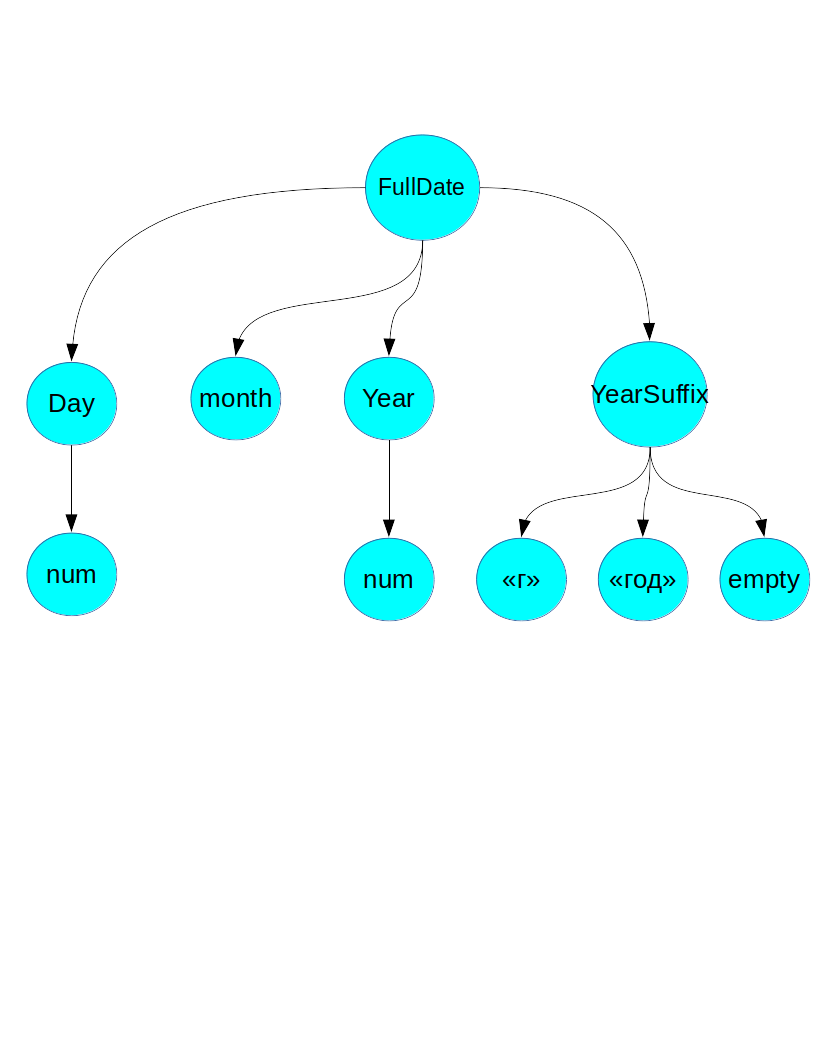
\includegraphics[width=\textwidth]{img/FullDateRule.png}
\caption{Граф отношения терминальных и нетерминальных слов в правиле FullDate}
\label{fig:FullDateRule}
\end{figure}

Теперь посмотрим, как происходит свертка терминальных и нетерминальных слов при разборе секции правил. Сначала рассмотрим случай с терминальным словом. За это отвечает метод \lstinline{handleTermReduction} в классе \lstinline{GParserDriver}.
\begin{Verb}
using PredArray = std::vector<PredicatePtr>;
GRuleWordPtr handleTermReduction(UnicodeString &&rawValue);
GRuleWordPtr handleTermReduction(UnicodeString &&rawValue, 
                                 PredArray &&predicates);
\end{Verb}
Как видно, есть две перегрузки этого метода: первая генерирует терминальное слово лишь на основе его имени, а вторая также обрабатывает список предикатов, связанных с терминалом. Посмотрим на реализацию второй перегрузки.
\begin{Verb}
GRuleWordPtr 
GParserDriver::handleTermReduction(UnicodeString &&rawValue, 
                                   PredArray &&predicates) 
{
    // получение терминала из пула
    auto term = GWordStorage::getTerminal(rawValue, predicates);
    // проверяем, не был ли он определен ранее
    auto termFound = terminals.find(term);
    if (termFound != terminals.end()) {
        return (*termFound);
    } else {
        terminals.insert(term);
        return term;
    }
}
\end{Verb}
Метод берет терминальное слово, соответствующее входному имени и набору предикатов, из специального пула, и затем проверяет, не был ли данный терминал определен ранее. Пул терминальных и нетерминальных слов был организован с целью упростить процедуру сравнения объектов класса \lstinline{GRuleWord}. Так как объекты полиморфные, то практически каждое сравнение предполагало интенсивное использование механизма RTTI (Run-Time Type Information), в частности, функции \lstinline{dynamic_cast}, что могло повлечь за собой негативное влияние на производительность, учитывая, что объекты типа \lstinline{GRuleWord} в программе очень часто сравниваются друг с другом на равенство. В конечном итоге было решено хранить указатели на эти объекты и сравнивать адреса. Благодаря этому сравнения с использованием RTTI производятся только на этапе разбора пользовательских правил. В дальнейшем на этапе поиска информационных полей сравниваются только адреса.

Пул реализован в рамках класса \lstinline{GWordStorage} и объявлен следующим образом:
\begin{Verb}
class GWordStorage {
public:
    using PredArray = vector<PredicatePtr>;
    using RWStorage = unordered_map<ReservedWord, UnicodeString>;

    static GRuleWordPtr getNonTerminal(const UnicodeString &name);
    static GRuleWordPtr getTerminal(const UnicodeString &name);
    static GRuleWordPtr getTerminal(const UnicodeString &name, 
                                    const PredArray &predicates);
    static GRuleWordPtr getEmptyTerminal();
    static GRuleWordPtr getEOITerminal();
    static GRuleWordPtr getNumTerminal();
private:
    static map<UnicodeString, GRuleWordPtr> nterms;
    static map<UnicodeString, vector<GRuleWordPtr>> terms;
};
\end{Verb}
Данный класс содержит методы получения объектов из пула, соответствующих терминальным и нетерминальным словам, включая специфические (например, \lstinline{getEmptyTerminal}). Также класс хранит список уже определенных объектов типа \lstinline{GRuleWord}. При запросе на доступ к объекту из пула первоначально происходит проверка, не был ли данный объект уже создан. Если был, то возвращаем его, иначе создаем.

Далее рассмотрим процесс свертки терминальных слов.
\begin{Verb}
GRuleWordPtr 
GParserDriver::handleNtermReduction(UnicodeString &&rawValue) {
    auto nterm = GWordStorage::getNonTerminal(rawValue);
    auto defFound = definedNterms.find(nterm);
    if (defFound != definedNterms.end()) {
        return (*defFound);
    }
    auto pendFound = pendingNterms.find(nterm);
    if (pendFound != pendingNterms.end()) {
        return *pendFound;
    }
    pendingNterms.insert(nterm);
    return nterm;
}
\end{Verb}
При свертке нетерминального слова мы получаем соответствующий объект \lstinline{GRuleWord} из пула. Далее мы проверяем, не был ли объект для данного нетерминала уже определен. Если был, то мы его извлекаем и возвращаем. В противном случае мы проверяем, не находится ли данный нетерминал в списке \lstinline{pendingNterms}, и если нет, то добавляем его туда. В \lstinline{pendingNterms} содержатся такие нетерминалы, которые встречались только в правых частях пользовательских правил и пока не были определены.

Рассмотрим теперь свертку правила. Вспомним еще раз синтаксис правил.
\begin{Verb}
simple_rule
    : CAPITAL_WORD ASSIGN rhs_chain
    ;
complex_rule
    : simple_rule
    | complex_rule DELIM rhs_chain
    ;
\end{Verb}
При свертке \lstinline{simple_rule} выполняется метод \lstinline{createRule} из класс \lstinline{GParserDriver}.
\begin{Verb}
GRuleWordPtr 
GParserDriver::createRule(UnicodeString &&word, 
                          std::vector<GRuleWordPtr> &&wordChain) 
{
    auto rule = GWordStorage::getNonTerminal(word);
    // сначала проверяем уже определенные нетерминалы
    auto defFound = definedNterms.find(rule);
    if (defFound != definedNterms.end()) {
        (*defFound)->getChildWords().push_back(wordChain);
        return *defFound;
    }
    // в том случае, если терминал еще не был
    // определен, проверяем pendingNterms
    auto pendFound = pendingNterms.find(rule);
    if (pendFound != pendingNterms.end()) {
        GRuleWordPtr pendPtr = *pendFound;
        pendingNterms.erase(pendFound);
        pendPtr->getChildWords().push_back(wordChain);
        return pendPtr;
    }
    // иначе добавляем в список определенных нетерминалов и
    // возвращаем как есть
    rule->getChildWords().push_back(wordChain);
    definedNterms.insert(rule);
    return rule;
}
\end{Verb}
В случае же свертки \lstinline{rhs_chain} после знака разделителя мы просто добавляем список объектов \lstinline{GRuleWord}, сформированных из \lstinline{rhs_chain}, в массив \lstinline{childWords} текущего нетерминала в левой части.

\subsection{Реализация разбора секции команд}
Разбор секции команд также происходит с помощью парсера, сгенерированного средствами GNU Bison. В результате разбора создается массив объектов класса \lstinline{DependencyGrammar}.
\begin{Verb}
struct DependencyGrammar {
    DependencyGrammar() = default;
    DependencyGrammar(const GRuleWordPtr &root);
    // указатель на грамматику
    std::shared_ptr<Grammar> grammar;
    // псевдоним
    UnicodeString alias;
    // список слов, определяющих контекст
    std::vector<UnicodeString> hintWords;
    // зависимости
    GrammarDepStorage dependencies;
};
\end{Verb}
\lstinline{DependencyGrammar} хранит указатель на объект, соответствующий грамматике, построенной для некоторого правила. Нужно уточнить, что подразумевается под грамматикой.

\begin{mydefinition}
Формальная грамматика $G$ определяется четверкой $(\Sigma, N, P, S)$Ё\autocite{formal-grammar}, где:
\begin{description}
  \item[$\Sigma$] алфавит терминальных символов.
  \item[$N$] алфавит нетерминальных символов.
  \item[$P$] множество правил вида $(\Sigma \cup N)^{*}N(\Sigma \cup N)^{*} \rightarrow (\Sigma \cup N)^{*}$.
  \item[$S$] стартовый символ, такой что $S \in N$.
\end{description}
\end{mydefinition}

\begin{mydefinition}
\label{def:ContextFreeGrammar}
Согласно иерархии Хомского~\autocite{homsky-hierarchy}, формальная грамматика относится к классу контекстно-свободных грамматик в том случае, когда все ее правила из множества $P$ имеют вид $N \rightarrow (\Sigma \cup N)^{*}$, где $P$ - множество правил грамматики, $N$ - множество нетерминальных символов, $\Sigma$ - множество терминальных символов.
\end{mydefinition}

Объект типа \lstinline{Grammar} описывает контекстно-свободную формальную грамматику. Чтобы в этом убедиться, приведем объявление класса \lstinline{Grammar}.
\begin{Verb}
class Grammar {
public:
    ...
private:
    ...
    std::set<GRuleWordPtr> terminals;
    std::set<GRuleWordPtr> nterminals;
    GRuleWordPtr root = nullptr;
};
\end{Verb}
Как видно, объявление данного класса включает в себя все атрибуты, которые свойственны формальной грамматике:
\begin{itemize}
  \item Поле \lstinline{terminals}, содержащее все терминальные слова, соответствует множеству $\Sigma$.
  \item Поле \lstinline{nterminals}, содержащее все правила, соответствует множеству $P$, а также множеству $N$ (так как класс \lstinline{GRuleWord} хранит, в том числе, имя правила).
  \item Поле \lstinline{root}, содержащее стартовое правило, соответствует символу $S$ (опять же, класс \lstinline{GRuleWord} хранит имя правила).
\end{itemize}

Теперь покажем, что класс \lstinline{Grammar} описывает контекстно-свободную грамматику. Вспомним объявление класса \lstinline{GRuleWord}, а также его производного класса - \lstinline{NonTerminal}.
\begin{Verb}
class GRuleWord {
    ...
    UnicodeString rawValue;
    ...
};
class NonTerminal final: public GRuleWord {
    ...
    std::vector<ChildWords> childWords;
    ...
};
\end{Verb}
Также вспомним, что правила в программе хранятся в виде объектов класса \lstinline{NonTerminal}. Мы видим, что данный класс содержит поле \lstinline{rawValue}, соответствующее элементу из множества $N$, а также список дочерних последовательностей терминальных и нетерминальных слов, каждый из которых, в свою очередь, также содержит поле \lstinline{rawValue}, значение которого принадлежит либо множеству $N$, либо множеству $\Sigma$. Таким образом, формат правила, который определен структурой класса \lstinline{NonTerminal}, соответствует формату правил из определения \ref{def:ContextFreeGrammar}. 

Более того, если мы вспомним формат записи пользовательских правил $Rule = rhs\_chain_1 | rhs\_chain_2 | \dots | rhs\_chain_n$, то увидим, что он соответствует форме Бэкуса-Наура~\autocite{backus-naur}.

Объекты класса \lstinline{DependencyGrammar} формируются в результате разбора и анализа секции команд. Данная секция содержит перечисление правил, согласно которым нужно извлекать информацию из документа, а также дополнительную информацию, которая позволяет задавать ограничения на контекст и расположения информации в тексте. Синтаксис и содержание секции команд были описаны в разделе \ref{subsect:CommandSection}. Объекты \lstinline{DependencyGrammar} формируются для каждой команды \lstinline{Find} и включают в себя:
\begin{itemize}
  \item Грамматику, сформированную из указанного в рамках команды \lstinline{Find} правила.
  \item Набор слов, определяющих контекст.
  \item Набор правил, определяющих зависимости.
  \item Псевдоним искомой сущности, который отобразится при выводе результатов.
\end{itemize}

Алгоритм обработки команды \lstinline{Find} следующий:
\begin{enumerate}
  \item Обработать правило и создать грамматику.
  \item Обработать слова, образующие контекст.
  \item Обработать правила, образующие зависимости.
  \item Обработать псевдоним.
\end{enumerate}

Метод \lstinline{handleCommandFindReduction} отвечает за обработку правила в рамках команды \lstinline{Find} и генерацию контекстно-свободной грамматики на его основе. Посмотрим на его реализацию:
\begin{Verb}
bool 
GParserDriver::handleCommandFindReduction(GRuleWordPtr &rule, 
                            DependencyGrammar &result, 
                            std::string &errMsg) 
{
    std::stringstream os;
    // осуществляем поиск правила в списке определнных
    auto ruleFound = definedNterms.find(rule);
    if (ruleFound == definedNterms.end()) {
        // если не определено - ошибка
        os << "Failed to find rule for " << rule;
        errMsg = os.str();
        return  false;
    }
    // проверяем, не было ли определено грамматики
    // для входного правила
    auto grammarFound = definedGrammars.find(rule);
    if (grammarFound != definedGrammars.end()) {
        result.grammar = grammarFound->second;
    } else {
        // если не было - создаем ее
        Grammar::GRuleWithInfo ruleWithInfo;
        ruleWithInfo.root = rule;
        extractTermsAndNterms(rule, 
                              ruleWithInfo.terms, 
                              ruleWithInfo.nterms);
        result.grammar = make_shared<Grammar>(ruleWithInfo);
    }
    result.alias = rule->getRawValue();
    return true;
}
\end{Verb}
При генерации грамматики входное правило трактуется как стартовое. Функция \lstinline{extractTermsAndNterms} осуществляет рекурсивный поиск всех терминальных и нетерминальных слов, которые встречаются в правой части входного правила либо же в правых частях дочерних правил.
\begin{Verb}
static void 
extractTermsAndNterms(const GRuleWordPtr &word,
                      std::set<GRuleWordPtr> &outTerms,
                      std::set<GRuleWordPtr> &outNterms)
{
    // если слово нетерминальное - тогда
    // рекурсивно проверяем все слова из childWords
    // и сохраняем его в массиве нетерминалов
    if (word->isNonTerminal()) {
        outNterms.insert(word);
        for (auto &ruleBody : word->getChildWords()) {
            for (auto &childWord : ruleBody) {
                if (word == childWord) {
                    continue;
                }
                extractTermsAndNterms(childWord, 
                                      outTerms, 
                                      outNterms);
            }
        }
    // иначе просто сохраняем слово
    // в массиве терминалов
    } else {
        outTerms.insert(word);
    }
}
\end{Verb}

После того, как мы получаем списки терминальных и нетерминальных слов, мы можем приступать к формированию грамматики. Конструктор грамматики принимает на вход объект типа \lstinline{GRuleWithInfo}.
\begin{Verb}
struct GRuleWithInfo {
    // стартовое правило
    GRuleWordPtr root;
    // нетерминальные слова
    std::set<GRuleWordPtr> nterms;
    // терминальные слова
    std::set<GRuleWordPtr> terms;
};
\end{Verb}
В конструкторе происходит инициализация грамматики: задается стартовое правило, множество терминальных и нетерминальных слов, множество правил.
\begin{Verb}
Grammar::Grammar(const Grammar::GRuleWithInfo &ruleWithInfo):
    root { ruleWithInfo.root },
    nterminals { ruleWithInfo.nterms },
    terminals { ruleWithInfo.terms }
{
    initAdditioanlParams();
}
void Grammar::initAdditioanlParams() {
    addExplicitRule();
    buildFirstSet();
    buildFollowSet();
}
\end{Verb}
Метод \lstinline{addExplicitRule} добавляет в грамматику искусственное стартовое правило \lstinline{S'}, в правую часть которого помещается текущее стартовое правило. Выглядит это так:
\begin{Verb}
void Grammar::addExplicitRule() {
  auto newRoot = make_shared<NonTerminal>(EXPLICIT_START_SYMBOL);
  newRoot->getChildWords().push_back({ root });
  root->getParentNterms().emplace_back(newRoot, 0, 0);
  root = newRoot;
  nterminals.insert(root);
}
\end{Verb}
После этого мы считаем, что грамматика сформирована.

На следующем шаге необходимо обработать слова, образующие контекст. За это отвечает метод \lstinline{handleHintWords}. Он получает на вход объект типа \lstinline{DependencyGrammar}, соответствующий текущей команде \lstinline{Find}, а также список слов, накопленный при разборе.
\begin{Verb}
void 
handleHintWords(DependencyGrammar &depRule, 
                std::vector<UnicodeString> &&hintWords) 
{
    depRule.hintWords = std::move(hintWords);
}
\end{Verb}

Далее нужно обработать зависимости. При свертке зависимости мы генерируем из нее грамматику и сохраняем в список, содержащий все зависимости в рамках текущей команды \lstinline{Find}. После того, как список будет окончательно сформирован, мы помещаем его в текущий объект \lstinline{DependencyGrammar}.
\begin{Verb}
using DependencyList = std::vector<std::shared_ptr<Grammar>>;

bool 
GParserDriver::handleDependencyReduction(DependencyList &depList, 
                                         GRuleWordPtr &dep, 
                                         std::string &errMsg) {
    // проверяем, что входное правило dep
    // уже было определено и генерируем из него грамматику 
    if (definedNterms.find(dep) == definedNterms.end()) {
        return false;
    }
    auto grammarFound = definedGrammars.find(dep);
    if (grammarFound != definedGrammars.end()) {
        depList.push_back(grammarFound->second);
    } else {
        Grammar::GRuleWithInfo ruleWithInfo;
        ruleWithInfo.root = dep;
        extractTermsAndNterms(dep, 
                              ruleWithInfo.terms, 
                              ruleWithInfo.nterms);
        depList.push_back(make_shared<Grammar>(ruleWithInfo));
    }

    return true;
}

void 
GParserDriver::processDependencies(DependencyGrammar &depRule, 
                                   GrammarDepStorage &&deps) 
{
    // сохраняем объект GrammarDepStorage
    depRule.dependencies = std::move(deps);
}
\end{Verb}

В рамках объекта \lstinline{DependepncyGrammar} зависимости хранятся в объекте типа \lstinline{GrammarDepStorage}. Зависимости в этом классе сгруппированы по пространственному признаку: левые, правые, верхние, нижние.
\begin{Verb}
template<class T>
struct DependencyStorage {
    std::vector<T> leftDeps;
    std::vector<T> rightDeps;
    std::vector<T> upperDeps;
    std::vector<T> lowerDeps;
};
using GrammarDepStorage = DependencyStorage<shared_ptr<Grammar>>;
\end{Verb}

Обработка псевдонима тривиальна: после его свертки получаем строку, которую затем сохраняем в объект \lstinline{DependencyGrammar}.
\begin{Verb}
void 
processAlias(DependencyGrammar &depRule, UnicodeString &alias) {
    if (!alias.isEmpty()) {
        depRule.alias = alias;
    }
}
\end{Verb}

Сформированные объекты \lstinline{DependencyGrammar} затем складываются в список \lstinline{targetGrammars}, который затем, вместе со списком токенов, подается на вход генератору GLR-парсеров.

\section{Извлечение информационных полей}
\subsection{Общая схема}
Накопленные на предыдущих этапах данные позволяют нам приступить непосредственно к извлечению информации из входного текста. Для каждой из грамматик, сформированных на этапе разбора пользовательских правил, мы строим таблицу разбора и, затем, производим разбор по алгоритму Томиты. Схема генерации таблицы переходов показана на рисунке \ref{fig:ParserTableGen}.
\begin{figure}% p означает, что нужно выделить для рисунка
% отдельную страницу; применяется для больших рисунков
\centering
%Здесь могла быть ваша лягушка.
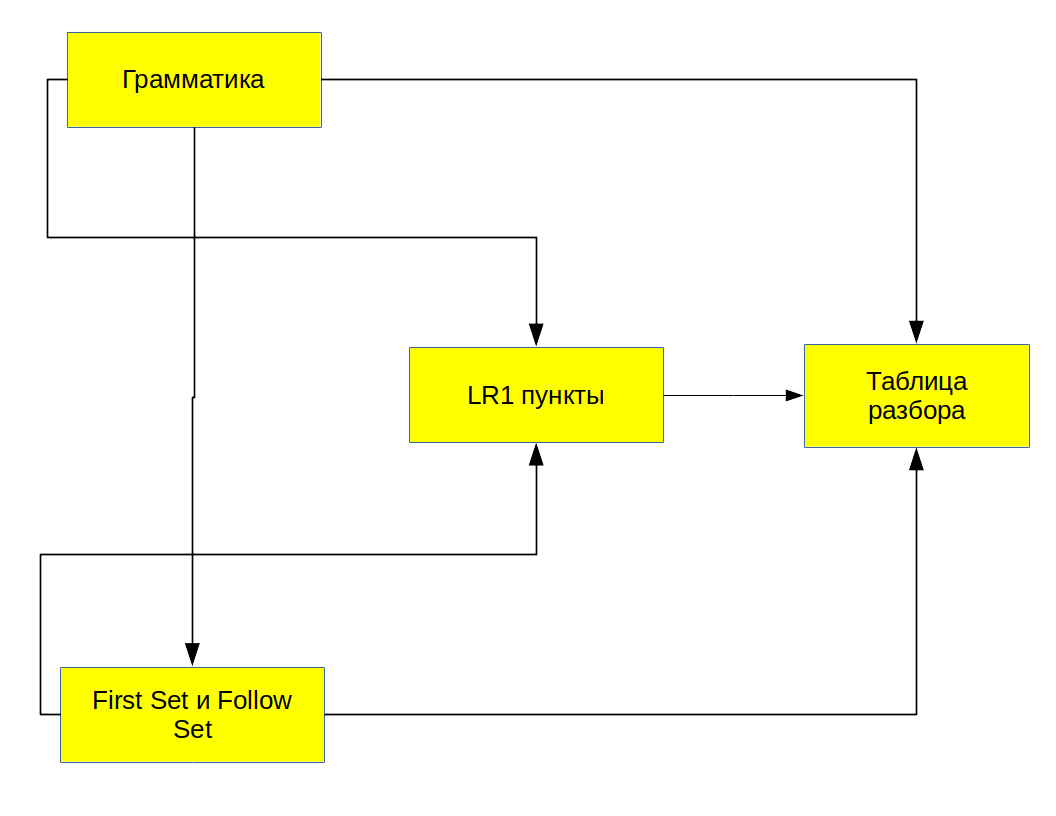
\includegraphics[width=\textwidth]{img/ParserTable.png}
\caption{Схема генерации таблицы переходов из грамматики}
\label{fig:ParserTableGen}
\end{figure}

В конечном итоге мы строим таблицу для SLR(1)-анализатора~\autocite{slr1}. Особенностью LR-анализатора является то, что он производит разбор слева направо, при этом его анализ является восходящим~\autocite{GLR-pars-algo}. Обыкновенно такой анализатор считывает токены с входного потока, накапливает их в специальной структуре данных - стеке, и проверяет уже накопленные токены на соответствие правой части какого-нибудь правила из грамматики. В том случае, если соответствие найдено, он снимает последние $N$ токенов со стека и помещает на их место левую часть соответствующего правила. Приведем пример.
\begin{myexample}
\label{examp:LRParser}
Пусть у нас есть следующая грамматика:\newline
S = S + S\newline
S = 1\newline
S = 0\newline
А также следующая строка:\newline
1 + 1 + 0\newline
Тогда процесс разбора данной строки с помощью LR1-анализатора будет происходить следующим образом:\newline
\begin{enumerate}
  \item Текущий входной символ: 1, стек пуст, действие: помещаем символ 1 на стек. Запрашиваем следующий токен на вход.
  \item Текущий входной символ: +, стек: 1. Содержимое стека соответствует правой части правила S = 1. Снимаем единицу, помещаем на стек S.
  \item Текущий входной символ +, стек: S. Помещаем <<+>> на стек. Запрашиваем следующий токен на вход.
  \item Текущий входной символ: 1, стек: S, +. Помещаем <<1>> на стек. Запрашиваем следующий токен на вход.
  \item Текущий входной символ: +, стек: S, +, 1. Содержимое стека соответствует правой части правила S = 1. Снимаем единицу, помещаем на стек S.
  \item Текущий входной символ: +, стек: S, +, S. Содержимое стека соответствует правой части правила S = S + S. Снимаем три последних символа, помещаем на стек S.
  \item Текущий входной символ: +, стек: S. Помещаем <<+>> на стек, запрашиваем следующий символ на вход.
  \item Текущий входной символ: 0, стек: S, +. Помещаем <<0>> на стек. Запрашиваем следующий символ на вход.
  \item Текущий символ: \$(конец строки), стек: S, +, 0. Содержимое стека соответствует правой части правила S = 0. Снимаем последний символ, помещаем на стек S.
  \item Текущий символ: \$(конец строки), стек: S, +, S. Содержимое стека соответствует правой части правила S = S + S. Снимаем три последних символа, помещаем на стек S.
  \item Текущий символ: \$(конец строки), стек: S. Достигли конца строки и на стеке стартовый символ. Строка распознана.
\end{enumerate}
\end{myexample}

Также существуют LL-анализаторы~\autocite{ll-parser}, которые производят нисходящий разбор. В начале разбора на стек помещается стартовый символ, и затем по входным токенам анализатор пытается понять, на правую часть из какого правила заменить содержимое стека.

Цифра 1 в аббревиатуре LR(1) означает, что в процессе разбора производится предпросмотр на 1 символ вперед~\autocite{slr1}. В частности, это позволяет производить свертку намного эффективнее за счет анализа так называемого Follow Set, который формируется для каждого нетерминального символа и в который помещаются все терминалы, которые могут встретиться непосредственно за данным нетерминалом. Использование Follow Set позволяет избежать части потенциальных конфликтов типа Shift/Reduce либо Reduce/Reduce. Приведем пример.
\begin{myexample}
Пусть у нас есть грамматика следующего вида:\newline
E = F\newline
E = E + F\newline
F = F * T\newline
F = T\newline
T = 1\newline
T = (E)\newline
И пусть у нас есть такая строка:
1 + 1 * 1
Процесс свертки показан на рисунке \ref{fig:WrongReduction}. Как видно, анализатор ошибочно произвел свертку в нетерминал E раньше времени. Если бы мы при свертке рассмотрели сперва множество Follow Set для нетерминала E, то увидели бы, что символа <<*>> там нет, и свертки бы не произошло.
\end{myexample}
\begin{figure}% p означает, что нужно выделить для рисунка
% отдельную страницу; применяется для больших рисунков
\centering
%Здесь могла быть ваша лягушка.
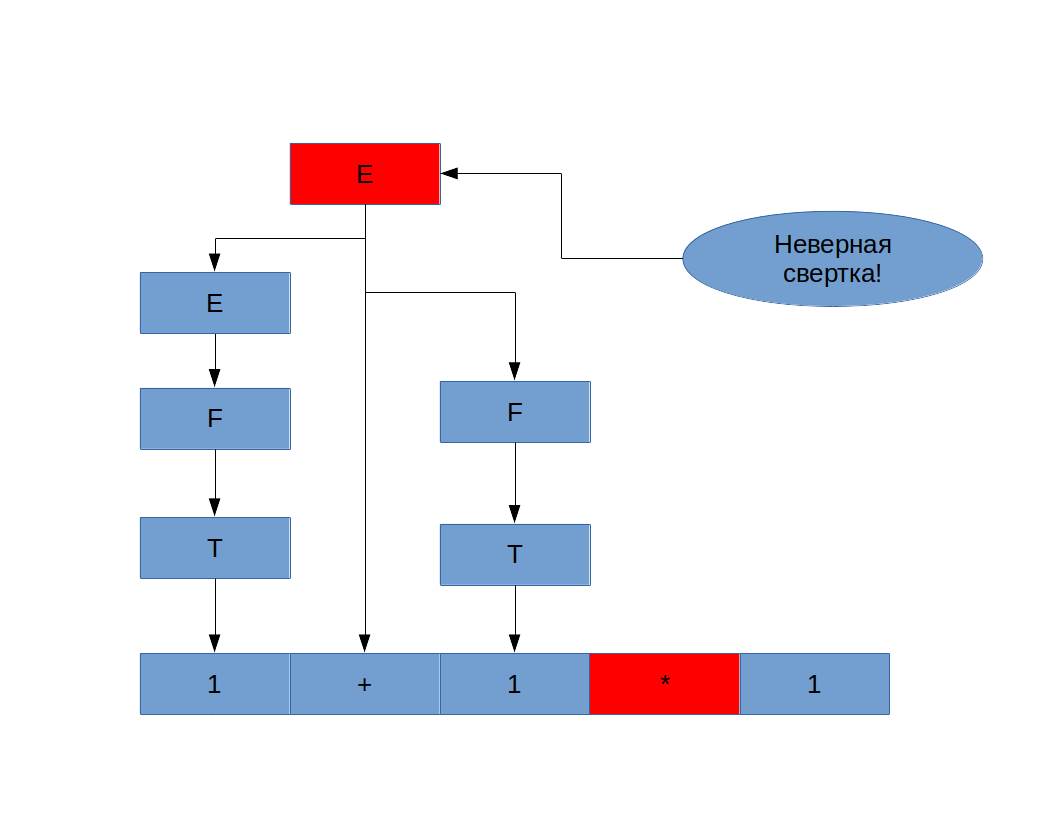
\includegraphics[width=\textwidth]{img/WrongReduction.png}
\caption{Пример ошибочной свертки при работе LR0-анализатора}
\label{fig:WrongReduction}
\end{figure}

\subsection{Построение множеств First и Follow}
Поскольку наш парсер будет осуществлять предпросмотр на один символ вперед, нам необходимо иметь в своем распоряжении множества First и Follow. 

Множество First строится для всех символов грамматики, включая терминальные и нетерминальные, по следующим правилам~\autocite{first-follow}:
\begin{enumerate}
  \item Если $X$ - терминал, то $First(X) = \{X\}$.
  \item Если существует правило $X \rightarrow \epsilon$, тогда добавляем $\epsilon$ в $First(X)$.
  \item Если существует правило $X \rightarrow Y_1Y_2...Y_k$, тогда добавляем $First(Y_1Y_2...Y_k)$ в $First(X)$.
  \item $First(Y_1Y_2...Y_k)$ - это:
  \begin{enumerate}
    \item $First(Y_1)$, если $\epsilon \notin First(Y_1)$.
    \item Либо же $First(Y_1Y_2...Y_k)$ содержит все элементы из $First(Y_1),First(Y_2),...First(Y_{m+1}), m < k$  за исключением $\epsilon$, если $\epsilon \in First(Y_1) \land \epsilon \in First(Y_2) \land \dots \land \epsilon \in First(Y_m)$.
    \item Если $\epsilon \in First(Y_1) \land \epsilon \in First(Y_2) \land \dots \land \epsilon \in First(Y_k)$, тогда $\epsilon \in First(Y_1Y_2...Y_k)$.
  \end{enumerate}
\end{enumerate}

Множество Follow строится в том числе на основе множества First. Алгоритм выглядит следующим образом~\autocite{first-follow}:
\begin{enumerate}
  \item Если $S$ - стартовый символ, тогда $\$ \in Follow(S)$, где $\$$ - символ конца строки.
  \item Если существует правило $A \rightarrow aBb$, тогда все из $First(b)$, за исключением $\epsilon$, помещается в $Follow(B)$.
  \item Если существует правило вида $A \rightarrow aB$, тогда $Follow(A) \in Follow(B)$.
  \item Если существует правило вида $A \rightarrow aBb$, причем $\epsilon \in First(b)$, тогда $Follow(A) \in Follow(B)$.
\end{enumerate}

\subsection{Реализация построения множеств First и Follow}
Множества First и Follow строятся сразу же после генерации грамматики. Хранятся они также в рамках объекта класса \lstinline{Grammar}.
\begin{Verb}
class Grammar {
    ...
    std::map<GRuleWordPtr, std::set<GRuleWordPtr>> firstSet;
    std::map<GRuleWordPtr, std::set<GRuleWordPtr>> followSet;
    ...
};
\end{Verb}

Построение First Set реализовано в рамках метода \lstinline{buildFirstSet}.
\begin{Verb}
void Grammar::buildFirstSet() {
    for (auto &terminal : terminals) {
        firstSet[terminal] = {terminal};
    }
    for (auto &nterminal : nterminals) {
        firstSet[nterminal] = firstSetForNonTerminal(nterminal);
    }
}
\end{Verb}
Сначала мы обрабатываем все терминальные слова, для которых $First(X) = \{X\}$. Далее мы приступаем к обработке нетерминальных слов.
\begin{Verb}
std::set<GRuleWordPtr> 
Grammar::firstSetForNonTerminal(const GRuleWordPtr &nterm) {
    std::set<GRuleWordPtr> firstSet;
    for (auto &childWords : nterm->getChildWords()) {

        if (childWords.size() == 1 && 
              childWords[0]->isEmptyWord()) 
        {
            firstSet.insert(childWords[0]);
        } else {
        ...
}
\end{Verb}
В рамках данного метода мы обрабатываем все ситуации, которые обговаривались в алгоритме построенная First Set. Первоначально мы обрабатываем ситуацию, при которой мы имеем правило вида $S \rightarrow \epsilon$. Далее мы рассчитываем First Set для правила вида $X \rightarrow Y_1Y_2...Y_k$.
\begin{ListingEnv}
\begin{lstlisting}[mathescape]
if (firstWord->isNonTerminal()) {
    bool shouldInsertEmptyWord = true;
    // cycle for $Y_1Y_2...Y_k$
    for (int i = 1; i <= childWords.size(); ++i ) {
        // calculate $First(Y_i)$
        auto result = firstSetForNonTerminal(firstWord);
        if (result.size() > 0) {
            int resultSize = result.size();
            result.erase(GWordStorage::getEmptyTerminal());
            // appending $First(Y_i)$ into $First(S)$
            firstSet.insert(result.begin(), result.end());
            // check if $\epsilon \in First(Y_i)$
            if (result.size() == resultSize) {
                shouldInsertEmptyWord = false;
                break;
            }
            firstWord = childWords[i];
        }
    }
    if (shouldInsertEmptyWord) {
        firstSet.insert(GWordStorage::getEmptyTerminal());
    }
} else {
    firstSet.insert(firstWord);
}
\end{lstlisting}
\caption{Расчет Follow Set для нетерминального слова}
\end{ListingEnv}

После того, как рассчитаны множества First для всех терминальных и нетерминальных слов, мы приступаем к расчету множества Follow. Множество Follow формируется в методе \lstinline{buildFollowSet}.
\begin{Verb}
void Grammar::buildFollowSet() {
    followSet[root] = { GWordStorage::getEOITerminal() };
    for (auto &nterm : nterminals) {
        if (nterm == root)
            continue;
        followSet[nterm] = followSetForNonTerminal(nterm);
    }
}
\end{Verb}
Первоначально мы инициализируем Follow Set для стартового правила \lstinline{root}. Затем мы высчитываем множество Follow для остальных нетерминалов. Происходит это в методе \lstinline{followSetForNonTerminal}.
\begin{Verb}
std::set<GRuleWordPtr> 
Grammar::followSetForNonTerminal(const GRuleWordPtr &word) 
{
    auto followForWord = followSet.find(word);
    if (followForWord != followSet.end()) {
        return  followForWord->second;
    }
    ...
}
\end{Verb}
Первоначально проверяем, что Follow Set не был построен ранее. Далее мы извлекаем информацию для текущего нетерминального слова относительно его расположения в правых частях других правил. Нас интересуют случаи $S \rightarrow aB$ и $S \rightarrow aBb$.
\begin{lstlisting}[mathescape]
for (auto infoRecord : wordIndexInfo) {
    GRuleWordPtr parentWord = infoRecord.nterm;
    auto ruleIndex = infoRecord.wordIndex.ruleIndex;
    auto &childWords = parentWord->getChildWords().at(ruleIndex);
    auto position = infoRecord.wordIndex.position;
    // $S \rightarrow aBb$ case
    if (position < childWords.size() - 1) {
        ...
        auto &nextWordFS = firstSet[nextWord];
        ...
        follow.insert(nextWordFS.begin(), nextWordFS.end());
        ... // if $\epsilon \in First(b)$
        {
            auto parentWordFS = followSetForNonTerminal(parentWord);
            follow.insert(parentWordFS.begin(), 
                          parentWordFS.end());
        }
    }
    // $S \rightarrow aB$ case
    else if (childWords[position] != parentWord) 
    {
        auto parentWordFS = followSetForNonTerminal(parentWord);
        follow.insert(parentWordFS.begin(), parentWordFS.end());
    }
}
\end{lstlisting}
После этого мы считаем, что множества First и Follow сформированы.

\subsection{Построение LR(0)-пунктов}
Этап построения LR(0)-пунктов является ключевым для формирования таблицы переходов. На этом этапе мы генерируем все возможные переходы из стартового правила, формируя наборы LR0-пунктов. Каждый набор соответствует состоянию в таблице переходов. Набор LR0-пунктов по сути содержит правила, в правой части каждого из которых зафиксирована определенная позиция. Эта позиция определяет тот символ, который мы можем встретить в текущем состоянии (иными словами, тот символ или слово, которое нам подадут на вход в процессе разбора). Из сформированной коллекции LR1 пунктов потом очень легко построить таблицу переходов. Пример такой коллекции приведен на рисунке \ref{fig:LRItems}.
\begin{figure}% p означает, что нужно выделить для рисунка
% отдельную страницу; применяется для больших рисунков
\centering
%Здесь могла быть ваша лягушка.
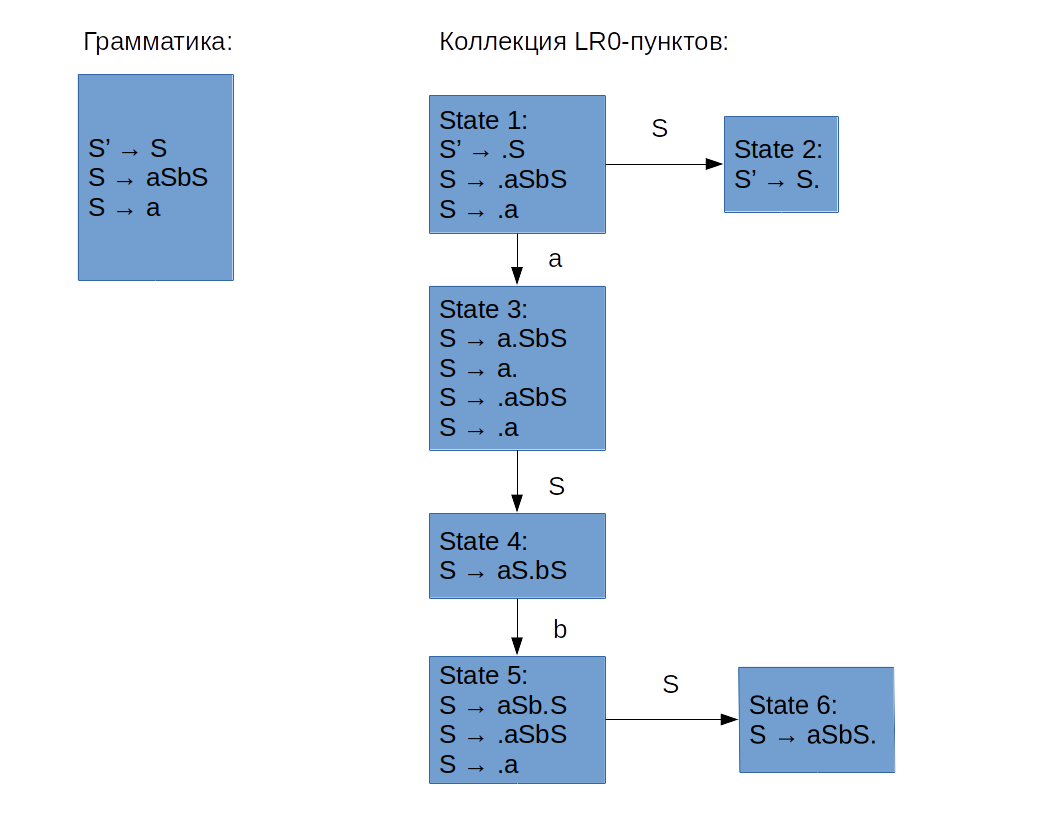
\includegraphics[width=\textwidth]{img/LRItems.png}
\caption{Пример коллекции LR0-пунктов для заданной грамматики}
\label{fig:LRItems}
\end{figure}

Построение коллекции LR0-пунктов происходит в несколько этапов~\autocite{lr-parsing}. Предполагается, что у нас имеется контекстно-свободная грамматика.
\begin{description}
  \item[Начальная операция] Пусть $S$ - стартовый символ грамматики и существует правило $S \rightarrow \alpha$. Тогда формируем начальный набор LR0-пунктов в виде $\{ S \rightarrow \cdot\alpha \}$.
  \item[Операция замыкания] Если существует LR0-пункт вида $S \rightarrow \alpha\cdot{B}\gamma$, где $B$ - нетерминальный символ, для некоторого состояния $I$, тогда все пункты вида $B \rightarrow \cdot\beta$ также нужно включить в состояние $I$. Данный этап нужно повторять для состояния $I$ до тех пор, пока не найдется новых пунктов для добавления.
  \item[Операция чтения] Пусть $A \rightarrow \alpha\cdot{X}\gamma$ пункт для некоторого состояния $I$, где $X$ - терминальный или нетерминальный символ. Тогда пункт $A \rightarrow \alpha{X}\cdot\gamma$ нужно поместить в состояние $J$, причем $J$ может быть эквивалентно $I$. Также нужно создать переход из $I$ в $J$ по $X$.
\end{description}

\subsection{Реализация построения коллекции LR0-пунктов}
Коллекция LR0-пунктов хранится в экземпляре класса \lstinline{LR0ItemSetCollection}.
\begin{Verb}
class LR0ItemSetCollection {
public:
    ...
    bool build(const Grammar &grammar);
private:
    ...
    std::vector<LR0ItemSet> itemSetCollection;
};
\end{Verb}
Данный класс характеризуется массивом объектов типа \lstinline{LR0ItemSet} и методом \lstinline{build}, который по входной грамматике строит коллекцию LR0-пунктов и сохраняет ее в массив \lstinline{itemSetCollection}. Класс \lstinline{LR0ItemSet} хранит в себе набор LR0-пунктов для конкретного состояния. Номер состояния в данном классе не хранится и берется для конкретного набора равным индексу этого набора в массиве \lstinline{itemSetCollection}.
\begin{Verb}
struct LR0ItemSet {
    ...
    std::vector<LR0Item> items;
    std::map<GRuleWordPtr, int> transitions;
    ...
};
\end{Verb}
Основное предназначение класса \lstinline{LR0ItemSet} хранить массив LR0-пунктов, представленных классом \lstinline{LR0Item}, а также список переходов в виде пар объектов \lstinline{GRuleWord} и \lstinline{int}, где первый соответствует слову, по которому осуществляется переход, а второй - состоянию, в которое мы попадаем по данному слову.
\begin{Verb}
struct LR0Item {
    GRuleWordPtr rule;
    WordIndex wordIndex;
    ...
};
\end{Verb}
Структура \lstinline{LR0Item} хранит в себе правило и индекс для текущего рассматриваемого слова в правой части правила.

Далее рассмотрим метод \lstinline{build} класса \lstinline{LR0ItemSetCollection}, который запускает процедуру построения коллекции LR0-пунктов.
\begin{Verb}
bool LR0ItemSetCollection::build(const Grammar &grammar) {
    history.clear();
    GRuleWordPtr root = grammar.getRoot();
    LR0ItemSet startItemSet;
    startItemSet.addItem({root, 0, 0});
    build(grammar, startItemSet, 0);
    return true;
}
\end{Verb}
В рамках данного метода мы инициализируем начальный набор LR0-пунктов, соответствующий начальному этапу их построения. Далее в дело вступает другой метод \lstinline{build}, который для входного объекта класса \lstinline{LR0ItemSet} производит операции замыкания и чтения. Если в результате был создан хотя бы один новый объект типа \lstinline{LR0ItemSet} (другими словами, если сформировался переход в такой набор LR0-пунктов, который ранее не рассматривался), то мы запускаем процедуру замыкания и чтения рекурсивно для всех таких новых объектов.

В конечно итоге мы получаем сформированную коллекцию LR0-пунктов в рамках класса \lstinline{LR0ItemSetCollection}.

\subsection{Построение анализатора SLR(0)}
После формирования коллекции LR0-пунктов построение таблицы переходов оказывается делом тривиальным. Вообще говоря, в результате осуществления данного этапа у нас получается не просто таблица, но конечный автомат. Вспомним определение конечного автомата.
\begin{mydefinition}
Конечный автомат задается пятеркой $(V, Q, q_0, F, \delta)$~\autocite{automation}, где:
\begin{description}
  \item[$V$] Входной алфавит.
  \item[$Q$] Множество состояний.
  \item[$q_0$] Начальное состояние, $q_0 \in Q$.
  \item[$F$] Множество допускающих состояний, $F \subset Q$.
  \item[$\delta$] функция переходов, определенная как отображение $\delta: Q \times (V \cup \{\epsilon\}) \rightarrow Q$.
\end{description}
\end{mydefinition}

\begin{mydefinition}
\label{def:ParserTable}
Допустим, что на входе у нас есть контекстно-свободная грамматика, множества First и Follow, а также коллекция LR0-пунктов. Тогда алгоритм построения таблицы переходов будет выглядеть следующим образом~\autocite{lr-parsing}:
\begin{enumerate}
  \item Пусть $C = \{I_0,I_1,...,I_n\}$ - коллекция LR0-пунктов для контекстно-свободной грамматики $G$.
  \item Строка таблицы, соответствующая состоянию $i$, конструируется из $I_i$. Действие при разборе для состояния $i$ определяется следующим образом:
  \begin{itemize}
    \item Если $A \rightarrow \alpha\cdot{a}\beta \in I_i$, $goto(I_i, a) = I_j$, и $a$ принадлежит множеству терминалов, тогда $action[i, a] = shift\ j$.
    \item $\text{Если}\ A \rightarrow \alpha\cdot \in I_i,$ тогда $action[i, a] = reduce\ A \rightarrow \alpha \allowbreak \forall a \in Folllow(A)$. Здесь мы используем возможность предпросмотра на один символ вперед, которую нам предоставляет множество Follow. Нетерминал $A$ не может быть стартовым символом.
    \item Если $S' \rightarrow S\cdot \in I_i$, тогда $action[i, \$] = accept$.
  \end{itemize}
  \item goto-переходы для состояния $i$ формируются для для всех нетерминалов $A$ по следующему правилу: если $goto(I_i, A) = I_j,$ тогда $goto[i, A] = j$.
  \item Все ячейки таблицы, не заполненные на шагах (2) и (3), помечаются как $error$.
\end{enumerate}
\end{mydefinition}

Теперь вернемся к обоснованию того, что на этом этапе мы строим автомат. Алфавитом входных символов $V$, очевидно, является объединение множеств терминальных и нетерминальных символов. Множество состояний $Q$ формируется в процессе алгоритма построения таблицы из коллекции LR0-пунктов, точно как описано в определении \ref{def:ParserTable}. Начальным состоянием является состояние, сконструированное из начального набора LR0-пунктов, то есть такого $I_i : S' \rightarrow \cdot{S} \in I_i$, где $S'$ - стартовый символ грамматики. Множество допускающих состояний являются все такие $i : action[i,a] = accept$, где $a$ - любое терминальное слово. И, наконец, функция $\delta$ задается таблицей переходов, построенной в результате алгоритма в определении \ref{def:ParserTable}.

\subsection{Реализация построения анализатора SLR(0)}
Построение анализатора осуществляется в рамках класс \lstinline{ParserTable}, который строит таблицу переходов по алгоритму из определения \ref{def:ParserTable} и определяет ряд методов для доступа к этой таблице.
\begin{Verb}
class ParserTable {
public:
    ...
    bool buildTableFromGrammar(const Grammar &grammar);
private:
    ...
    ActionTablePtr actionTable {nullptr};
    GotoTablePtr gotoTable {nullptr};
};
\end{Verb}
Построение таблицы происходит в рамках метода \lstinline{buildTableFromGrammar}, который принимает на вход объект типа \lstinline{Grammar}. В результате вызова этого метода мы получаем сформированную таблицу переходов, которая разбита на два двумерных массива: \lstinline{actionTable} и \lstinline{gotoTable}. Первый хранит переходы для всех терминальных слов, второй - для нетерминальных. Реализация метода \lstinline{buildTableFromGrammar} представляет собой поэтапное выполнение алгоритма из определения \ref{def:ParserTable}. Мы итерируемся по всем наборам LR0-пунктов и проверяем все ситуации, описанные в алгоритме. Первым делом мы заполняем таблицу \lstinline{actionTable}.
\begin{lstlisting}[mathescape]
for (auto &item : currentItemSet) {
    // check $A \rightarrow \alpha\cdot$ case
    if (item.atEndPosition()) {
        std::set<GRuleWordPtr> followWords;
        if (grammar.followWords(item.rule,followWords)) {
            ...
            for (auto &followWord : followWords) {
                // check $S' \rightarrow S\cdot$ case
                if (followWord->isEndOfInput() && 
                    item.rule == grammar.getRoot()) {
                    addNewAction(i, 
                          followWord, 
                          make_shared<ParserAction>(ACCEPT));
                } else {
                    addNewAction(i, 
                          followWord, 
                          make_shared<ReduceAction>(ruleIndex));
                }
            }
        } else {
            return false;
        }
    } else {
        // this is just $A \rightarrow \alpha\cdot{a}\beta$ case
        GRuleWordPtr nextWord = item.getCurrentWord();
        if(!nextWord->isNonTerminal()) {
            int next = currentItemSet.getNextState(nextWord);
            addNewAction(i, 
                    nextWord,
                    std::make_shared<ShiftAction>(next));
        }
    }
}
\end{lstlisting}

Далее мы приступаем к заполнению таблицы \lstinline{gotoTable}.
\begin{lstlisting}
auto transitions = currentItemSet.getTransitions();
std::map<GRuleWordPtr, int> ntermTransitions;
for (auto &transition : transitions) {
    if (transition.first->isNonTerminal()) {
        ntermTransitions.insert(transition);
    }
}
(*gotoTable)[i] = std::move(ntermTransitions);
\end{lstlisting}
Здесь мы проверяем все переходы для текущего набора LR0-пунктов и обрабатываем такие, для которых символ перехода является нетерминальным словом.

Итак, по итогам данного этапа у нас сформирован анализатор в виде конечного автомата. После этого мы можем приступать непосредственно к алгоритму разбора.

\subsection{Алгоритм GLR-разбора}
Для разбора текста на естественном языке было решено применить алгоритм GLR-разбора, разработанный японским ученым Масару Томитой. Данный алгоритм хорошо подходит для анализа естественного языка, так как позволяет справляться с конфликтами типа Shift/Reduce и Reduce/Reduce. Такие конфликты неизбежно возникают в силу многозначной трактовки многих конструкций естественного языка. Приведем простейший пример такой ситуации.
\begin{myexample}
Name = word(type: name)\newline
Noun = word(type: noun)\newline
Эти два правила определяют сущности <<имя>> и <<имя существительное>>. Однако же, они не являются взаимоисключающими: и одно и то же слово может быть и тем, и другим. Классический алгоритм LR-разбора не сможет корректно разрешить такую ситуацию.
\end{myexample}

Классический алгоритм LR-разбора главным образом оперирует таким понятием, как стек. Весь процесс построен вокруг него. Стек содержит два вида узлов: символьные узлы и узлы, обозначающие состояния. Если стек не пуст, то на его вершине всегда узел состояния. Таким образом мы определяем текущее состояние при разборе. Разбор включает в себя два основных действия:
\begin{description}
  \item[Shift или сдвиг] Данное действие осуществляется в том случае, когда существует $action[i, a] = shift\ j$, где $i$ - текущее состояние на вершине стека, $a$ - текущий входной символ, $j$ - состояние, в которое мы попадем в результате перехода. Мы помещаем на стек символьный узел $a$, затем узел состояния $j$, который оказывается на вершине, и запрашиваем следующий символ на вход.
  \item[Reduce или свертка] Данное действие осуществляется в том случае, когда существует $action[i, a] = reduce\ A$, где $i$ - текущее состояние на вершине стека, $a$ - текущий входной символ, $A$ - правило, по которому нужно осуществить свертку. Мы снимаем со стека символы в количестве равном $2 * |rhs(A)|$, после чего на вершине оказывается состояние $k$. Далее мы считываем из таблицы $goto$ ячейку, соответствующую состоянию $k$ и нетерминалу $A$. Если $goto[k, A] = r$, тогда мы помещаем на стек символьный узел $A$ и узел состояния $r$, который оказывается на вершине.
\end{description}
Конфликты возникают, когда $action[i, a]$ содержит более одного действия.

Существует грубый метод, являющийся модификацией приведенного выше алгоритма и позволяющий разрешать конфликты типа Shift/Reduce и Reduce/Reduce. Он заключается в том, чтобы полностью копировать стек каждый раз, когда возникают конфликты. Например, если $action[i, a] = \{shift\ j,\ reduce\ A\}$, тогда текущий стек будет продублирован, и после этого для одного из стеков мы произведем свертку. Далее мы синхронно продолжим сдвиг (стеки синхронизируются именно по сдвигу). Соответственно, считается, что анализатор допустил входную последовательность тогда, когда хотя бы по одному из стеков мы пришли в финальное состояние.

Данный подход неэффективен, так как нередко возникают ситуации, когда два или более стеков в конечном итоге приходят в одно и то же состояние, после чего мы фактически дублируем одни и те же действия несколько раз. Кроме того, отсутствие механизма слияния стеков может вызывать очень быстрый рост их количества при разборе.

Томита предложил алгоритм разбора, основанный на новой структуре данных под названием Graph Structured Stack (GSS). Данный алгоритм позволяет избежать вышеописанных проблем в процессе разбора при использовании неоднозначных грамматик, содержащих конфликты. Суть алгоритма Томиты в том, что он не дублирует стек полностью, но разветвляет лишь необходимую его часть. Кроме того, предусмотрен механизм слияния тех стеков, что пришли в одно и то же состояние.

Graph Structred Stack - центральная структура данных для алгоритма GLR-разбора. По своей сути она является направленным ациклическим графом, содержащим два вида узлов: символьный узел и узел состояния. Символьные узлы помечаются терминальными и нетерминальными символами грамматики, а узлы состояния - номерами состояний анализатора. Узлы состояния сгруппированы в $N + 1$ не пересекающихся множеств, которые называют уровнями. GSS строится по одному уровню за раз. Сначала производятся все возможные свертки для узлов из текущего уровня (фронта), затем формируется следующий уровень как результат применения операции сдвига. Первый уровень инициализируются из начального состояния анализатора.

\begin{figure}% p означает, что нужно выделить для рисунка
% отдельную страницу; применяется для больших рисунков
\centering
%Здесь могла быть ваша лягушка.
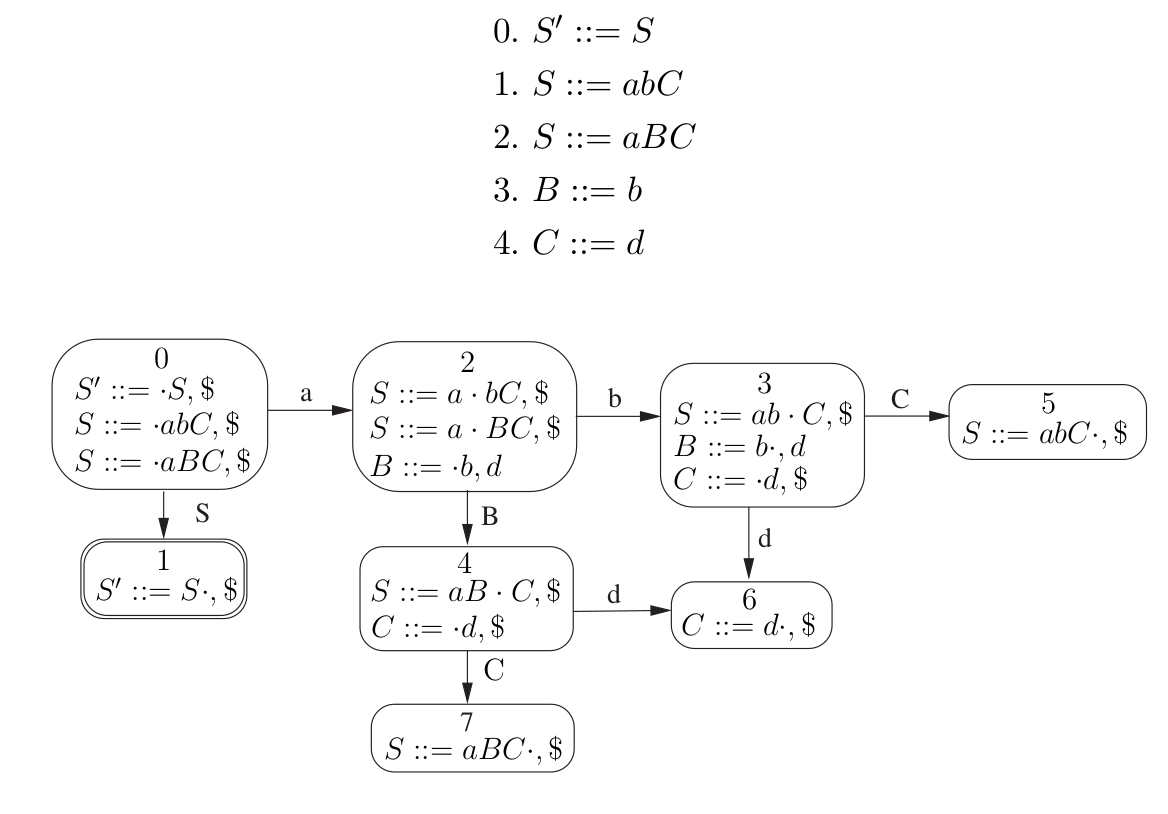
\includegraphics[width=\textwidth]{img/glr-sample-grammar.png}
\caption{Пример неоднозначной грамматики, содержащей конфликты}
\label{fig:AmbigiousGrammar}
\end{figure}

\begin{figure}% p означает, что нужно выделить для рисунка
% отдельную страницу; применяется для больших рисунков
\centering
%Здесь могла быть ваша лягушка.
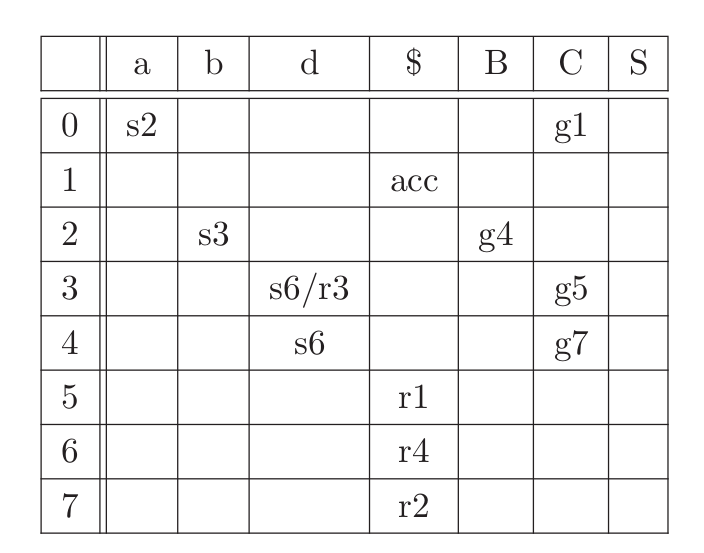
\includegraphics[width=\textwidth]{img/glr-parser-table.png}
\caption{Таблица разбора для грамматики из рисунка \ref{fig:AmbigiousGrammar}}
\label{fig:AmbigiousParserTable}
\end{figure}

Далее рассмотрим пример работы алгоритма GLR-разбора Томиты. Пусть у нас есть грамматика из рисунка \ref{fig:AmbigiousGrammar} и таблица разбора из рисунка \ref{fig:AmbigiousParserTable}, а также входное слово $abd$. GSS инициализируется узлом, обозначающим начальное состояние, - $u_0$ на уровне $U_0$. Далее на вход поступает символ $a$ и мы совершаем сдвиг согласно $action[0, a] = shift\ 2$, формируя новый уровень $U_1$.
\begin{figure}[H]
\centering
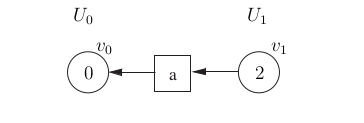
\includegraphics[width=0.5\textwidth]{img/gss-step1.png}
\end{figure}

После этого на вход поступает символ $b$ и мы анализируем соответствующую ячейку таблицы - она содержит $action[2, b] = shift\ 3$. Мы осуществляем сдвиг и формируем новый уровень $U_3$.
\begin{figure}[H]
\centering
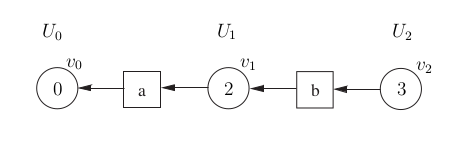
\includegraphics[width=0.5\textwidth]{img/gss-step2.png}
\end{figure}

Далее на вход поступает символ $d$ и мы получаем конфликт типа Shift/Reduce, так как $action[3, d] = \{shift\ 6,\ reduce B \rightarrow b\}$. Поскольку построение GSS синхронизируется по сдвигу, то мы запоминаем текущий сдвиг и приступаем к осуществлению свертки. В отличие от стандартного алгоритма LR-разбора, который снимает со стека узлы при осуществлении свертки, в рамках данного алгоритма при свертке мы находим все пути на графе длины $2 *|rhs(B)|$ из текущего узла. В данной ситуации имеется только один путь, который ведет в узел $u_2$. После этого мы находим соответствующую запись в таблице переходов $goto[2, B] = 4$. Добавляем в GSS два новых узла: символьный узел, соответствующий нетерминалу $B$ и узел состояния, соответствующий состоянию 4, который добавляем в текущий фронт (уровень $U_2$).
\begin{figure}[H]
\centering
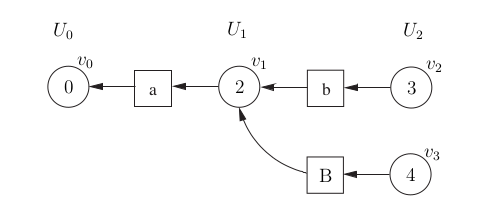
\includegraphics[width=0.5\textwidth]{img/gss-step3.png}
\end{figure}

Поскольку мы обработали все узлы на уровне $U_2$ и все свертки для них произведены, то мы можем приступать к формированию следующего уровня $U_3$ путем осуществления сдвигов для узлов $u_2$ и $u_3$. Следующий входной символ $d$, и действия в таблице следующие: $action[3, d] = shift\ 6$, $action[4, d] = shift\ 6$. Оба сдвига ведут в состояние 6, поэтому при создании уровня $U_3$ мы можем произвести слияние стека.
\begin{figure}[H]
\centering
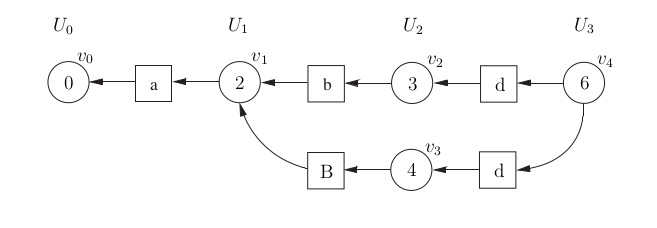
\includegraphics[width=0.8\textwidth]{img/gss-step4.png}
\end{figure}

Прежде, чем приступить к формированию следующего уровня, нужно осуществить все возможные свертки. Поскольку мы достигли конца строки, то проверяем символ $\$$. В таблице переходов мы видим запись в соответствующей ячейке: $action[6, \$] = reduce\ C \rightarrow d$. Теперь нам нужно найти все пути на графе длина $|rhs(C)|$, ведущие из состояния 6. Таких путей два: один ведет в вершину $u_3$, другой - в вершину $u_4$. Нам нужно обработать оба этих пути. Для состояния 3 и нетерминала $C$ есть переход, ведущий в состояние 5, а для состояния 4 и нетерминала $C$ - переход в состояние 7. Обновим теперь уровень $U_3$.
\begin{figure}[H]
\centering
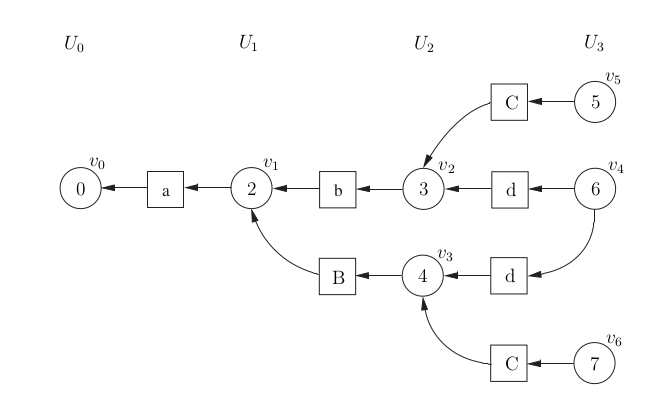
\includegraphics[width=0.8\textwidth]{img/gss-step5.png}
\end{figure}

Проанализировав узлы $u_5$ и $u_6$, мы видим, что оба они для входного символа $\$$ имеют в таблице переходов свертку по правилам $S \rightarrow abC$ и $S \rightarrow aBC$, для которых $2 * rhs == 6$. Осуществим поиск путей длины шесть из данных узлов, после чего заметим, что оба ведут в узел $u_0$. Обновим наш GSS соответствующим образом. 
\begin{figure}[H]
\centering
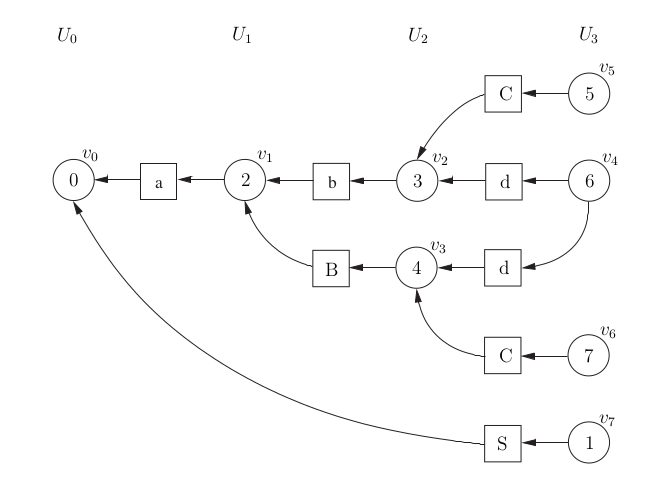
\includegraphics[width=0.8\textwidth]{img/gss-step6.png}
\end{figure}

Проанализировав узел $u_7$, мы видим переход $action[1, \$] = accept$. Поскольку мы обработали все входные символы, а также проанализировали все узлы из текущего уровня, то мы считаем, строка $abd$ допущена парсером.

\subsection{Реализация алгоритма GLR-разбора}
В основе алгоритма Томиты лежит Graph Structured Stack, который имеет два вида узлов: узлы состояния и символьные. Узел GSS реализован в рамках структур \lstinline{GSSNode}.
\begin{Verb}
struct GSSNode {
    virtual std::set<GSSNodePtr> getSucc() const = 0;
    virtual void addSucc(const GSSNodePtr &node) = 0;
    virtual ~GSSNode() {}
};
\end{Verb}
Это абстрактный класс, в котором объявлен общий для обоих типов узлов функционал - работа с узлами потомками, их добавление и считывание. Каждый объект класса \lstinline{GSSNode} хранит в себе указатели на один или несколько узлов-потомков.

Символьный узел реализован в рамках класса \lstinline{GSSSymbolNode}.
\begin{Verb}
struct GSSSymbolNode : public GSSNode, private GSSNodePrivate {
    GSSSymbolNode(const UnicodeString &word);
    UnicodeString word;
    std::set<GSSNodePtr> getSucc() const override;
    void addSucc(const GSSNodePtr &node) override;
};
\end{Verb}
Данный класс дополнительно содержит информацию о хранимом терминальном или нетерминальном слове.

Узел состояния хранится в рамках класса \lstinline{GSSStateNode}.
\begin{Verb}
struct GSSStateNode : public GSSNode, private GSSNodePrivate {
    GSSStateNode(int state);
    int state;
    std::set<GSSNodePtr> getSucc() const override;
    void addSucc(const GSSNodePtr &node) override;
};
\end{Verb}
Данный класс дополнительно содержит информацию о номере состояния.

Для узлов типа \lstinline{GSSNode} также реализовано две вспомогательные функции:
\begin{Verb}
std::vector<GSSNodePtr> 
findAllDestsForPath(const GSSNodePtr &node, int pathLength);

bool 
isExistsPath(const GSSNodePtr &startNode, 
             const GSSNodePtr &destNode);
\end{Verb}
Первая возвращает список конечных узлов для всех путей длины \lstinline{pathLength} из узла \lstinline{node}. Вторая проверяет существование пути из узла \lstinline{startNode} в узел \lstinline{destNode}.

Алгоритм GLR-разбора реализован в рамках класса \lstinline{Parser}.
\begin{Verb}
class Parser {
public:
    Parser(const std::shared_ptr<Grammar> &grammar, 
           const ParserTable &parserTable);
    bool tryParse(const Tokenizer::Sentence &sentence, 
          std::vector<std::pair<UnicodeString,int>> &result);
    ...
};
\end{Verb}
Данный класс при инициализации принимает на вход грамматику и таблицу переходов. Процесс разбора запускается в рамках метода \lstinline{tryParse}.
\begin{Verb}
while (sentenceBegin != sentence.end()) {
    UnicodeString currentChain;
    int position = -1;
    for (auto it = sentenceBegin; it != sentence.end(); ++it) {
        currentSet = parseToken(*it, currentSet, isAccepted);
        if (isAccepted || 
            currentSet.size() == 0 || 
            it == sentence.end() - 1) 
        {
            if (isAccepted) {
                result.push_back({currentChain, position});
                isAccepted = false;
            }
            currentSet = {std::make_shared<GSSStateNode>(0)};
            sentenceBegin++;
            break;
        } else if (currentSet.size() > 0) {
            if (currentChain.isEmpty()) {
                position = it - sentence.begin();
            }
            currentChain.append(it->word + " ");
        }
    }
}
\end{Verb}
В данном методе мы проходим по всем токенам из поданного на вход объекта типа \lstinline{Sentence} (который соответствует абзацу) и поочередно подаем их на вход анализатору, при этом проверяя множество \lstinline{currentSet}, которое соответствует фронту. Если множество не пусто, то мы двигаемся дальше, иначе отбрасываем начальный токен и перезапускам процесс разбора.

Метод \lstinline{parseToken} реализует разбор для входного токена.
\begin{Verb}
Parser::ActiveSet 
Parser::parseToken(const Token &token, 
                   ActiveSet &currentLevelSet, 
                   bool &accepted) 
{
    ActiveSet activeNodes = currentLevelSet;
    ActiveSet nextLevelNodes;
    ReduceSet reduceSet;
    ShiftSet shiftSet;
    while (reduceSet.size() > 0 || 
           activeNodes.size() > 0) 
    {
        if (activeNodes.size() > 0) {
            actor(token, 
                  activeNodes, 
                  reduceSet, 
                  shiftSet, 
                  accepted);
        }
        if (reduceSet.size() > 0) {
            reducer(token, 
                    activeNodes, 
                    currentLevelSet, 
                    reduceSet);
        }
    }
    shifter(nextLevelNodes, shiftSet);
    return nextLevelNodes;
}
\end{Verb}
В рамках данного метода реализована обработка узлов из фронта (\lstinline{activeNodes}). Метод \lstinline{actor} проходит по всем активным узлам и накапливает действия, которые для них применимы согласно таблице переходов: действия, связанные со сверткой, накапливаются в \lstinline{reduceSet}, а действия, связанные со сдвигом, - в \lstinline{shiftSet}. Метод \lstinline{reducer} выполняет все накопленные в \lstinline{reduceSet} свертки для узлов из текущего фронта. Мы продолжаем анализ новых узлов, если таковые появляются. Если же мы выполнили все возможные свертки, тогда выполняется метод \lstinline{shifter}, который обрабатывает все накопленные во множестве \lstinline{shiftSet} сдвиги, формируя следующий уровень.

В методе \lstinline{tryParse} происходит накопление токенов. Мы сохраняем токен в том случае, если его обработка в методе \lstinline{parseToken} привела к формированию нового непустого уровня в структуре GSS. Мы заканчиваем накопление и сохраняем результат в том случае, когда метод \lstinline{actor} обнаружил финальное состояние и выставил соответствующий флаг.

\chapter{Примеры работы программы}
\section{Пример 1}
Рассмотрим пример извлечения полей полей, соответствующих полному имени нанимателя и адреса помещения, которое предоставляется в аренду.
\begin{myexample}[Отрывок текста из договора об аренде]
Договор найма жилого помещения № 112\\
г. Ростов-на-Дону «19» августа 2015 г.\\ 
Гражданин Иванов Иван Иванович, паспорт (серия, номер, выдан) 6545 033655, именуемый в дальнейшем "Наймодатель", с одной стороны, и гражданин Петров Петр Петрович, паспорт (серия, номер, выдан) 6565 033654, именуемый в дальнейшем "Наниматель", с другой стороны, именуемые в дальнейшем «Стороны», заключили настоящий договор, в дальнейшем «Договор», о нижеследующем:\\ 
1. ПРЕДМЕТ НАСТОЯЩЕГО ДОГОВОРА\\
1.1. Наймодатель предоставляет Нанимателю помещение, состоящее из трех комнаты, (в трехкомнатной квартире) расположенное по адресу город Ростов-на-Дону, улица Волкова, дом 5, квартира 184 за плату, во временное пользование в целях проживания. \\
...
\end{myexample}
\begin{myexample}[Правила, описывающие искомые поля]
\label{rules1}
\begin{Verb}
%rules
Address = Town Street;
%commands
Find PersonFullName (hint_words: "наниматель") as Employer;

Find Address (hint_words: "располагаться", "находиться", "адрес") 
as ApartementAddress;
\end{Verb}
\end{myexample}

В результате работы программы мы получим следующий вывод:
\begin{Verb}
Extraction result:
Field name: ApartementAddress
Field value: город Ростов-на-Дону улица Волкова дом 5 
Field name: Employer
Field value: Петров Петр Петрович 
Press <RETURN> to close this window...
\end{Verb}

Рассмотрим еще один договор, который содержит в себе текст, приведенный в примере \ref{agr1}.
\begin{myexample}[Отрывок из договора об аренде]
\label{agr1}
Договор найма жилого помещения\\

г. Ростов-на-Дону \                                                        «12» июня 2017 г.\\

     Гражданин Меркулов Сергей Андреевич, именуемый в дальнейшем «Наймодатель»,  личность  удостоверяется  паспортом: 0505  634888, выданным 11 мая 2010 года Паспортным столом № 12312312312, код подразделения 56, проживающий по адресу: г. Петропавловск-Камчатский, ул. Ленина дом 115 кв. 22 с одной стороны, и гражданин Меркулов Андрей Андреевич, именуемый в дальнейшем «Наниматель»,  личность  удостоверяется  паспортом:   0505  634888,  выданным 15 июля 2013 года паспортным столом № 1321312312, код подразделения 546, проживающий по адресу: Россия, г. Братск, ул. Вавилова дом 11 кв. 25, заключили настоящий договор, далее «Договор»,  на следующих условиях:\\

1. ПРЕДМЕТ ДОГОВОРА\\
\\
1.1. По настоящему договору Наймодатель предоставляет принадлежащую ему на праве собственности квартиру Нанимателю за плату во владение и пользование для проживания в ней.\\
1.2. Указанная квартира находится по адресу: г. Петропавловск-Камчатский, ул. Ленина дом 115 кв. 23.\\
1.3. Право собственности Наймодателя на указанную квартиру подтверждается следующими документами: .\\
1.4. Наниматель использует квартиру в течение всего срока найма в соответствии с ее целевым назначением (для проживания).\\
1.5. Вместе с Нанимателем в квартире, указанной в п. 1.2 Договора, будут совместно проживать и иметь равные с Нанимателем права по пользованию жилым помещением следующие граждане:\\
...
\end{myexample}
Применим к нему правила из примера \ref{rules1} и увидим такой вывод:
\begin{Verb}
Extraction result:
Field name: ApartementAddress
Field value: г Петропавловск-Камчатский ул Ленина дом 115 
Field name: Employer
Field value: Меркулов Андрей Андреевич 
Press <RETURN> to close this window...
\end{Verb}

\section{Пример 2}
Теперь будем искать поля, описанные в примере \ref{rules2}.
\begin{myexample}[Правила извлечения полей]
\label{rules2}
\begin{Verb}
%rules
PassportSeries = num(len: 4);
Fee = num(len: 4...6);
%commands
Find FullDate with deps (left: Town) 
as AgreementDateValue;

Find PassportSeries (hint\_words: "наймодатель") 
as OwnerPassportSeries;

Find FullDate (hint\_words: "период", "до", "срок") 
as RentEndPeriod;

Find Fee (hint\_words:"ежемесячно", "месячный", "рубль") 
as RentFee;
\end{Verb}
\end{myexample}

\begin{myexample}[Отрывок из текста договора об аренде]
\label{agr12}
Договор найма жилого помещения № 112\\
г. Ростов-на-Дону «19» августа 2015 г.\\ 
Гражданин Иванов Иван Иванович, паспорт (серия, номер, выдан) 6545 033655, именуемый в дальнейшем "Наймодатель", с одной стороны, и гражданин Петров Петр Петрович, паспорт (серия, номер, выдан) 6565 033654, именуемый в дальнейшем "Наниматель", с другой стороны, именуемые в дальнейшем «Стороны», заключили настоящий договор, в дальнейшем «Договор», о нижеследующем: \\
1. ПРЕДМЕТ НАСТОЯЩЕГО ДОГОВОРА\\
1.1. Наймодатель предоставляет Нанимателю помещение, состоящее из трех комнаты, (в трехкомнатной квартире) расположенное по адресу город Ростов-на-Дону, улица Волкова, дом 5, квартира 184 за плату, во временное пользование в целях проживания. \\
1.2. Помещение принадлежит Наймодателю на основании статьи №113.\\
1.3. В течение всего срока найма совместно с Нанимателем в квартире будут проживать:\\
1.4. Срок найма указанного помещения устанавливается с «10» апреля 2010 года по «11» мая 2015 года.\\
1.5. В случае согласия сторон, срок Договора продлевается самостоятельно. \\
...\\
3. ПЛАТЕЖИ И РАСЧЕТЫ\\
3.1. Месячная оплата за использование помещения составляет 2000 (две тысячи) рублей.\\
3.2. В дальнейшем оплата будет производиться ежемесячно, далее не позднее 15 числа каждого текущего месяца.\\ 
3.3. В качестве гарантийного платежа (залога), Нанимателем внесена сумма в размере 5000 (пять тысяч) рублей.\\
\end{myexample}

\begin{myexample}[Отрывок из текста договра об аренде]
\label{agr22}
Договор \\
найма жилого помещения\\

г. Ростов-на-Дону               \                                          «12» июня 2017 г.\\

     Гражданин Меркулов Сергей Андреевич, именуемый в дальнейшем «Наймодатель»,  личность  удостоверяется  паспортом: 0505  634888, выданным 11 мая 2010 года Паспортным столом № 12312312312, код подразделения 56, проживающий по адресу: г. Петропавловск-Камчатский, ул. Ленина дом 115 кв. 22 с одной стороны, и гражданин Меркулов Андрей Андреевич, именуемый в дальнейшем «Наниматель»,  личность  удостоверяется  паспортом:   0505  634888,  выданным 15 июля 2013 года паспортным столом № 1321312312, код подразделения 546, проживающий по адресу: Россия, г. Братск, ул. Вавилова дом 11 кв. 25, заключили настоящий договор, далее «Договор»,  на следующих условиях:\\
...\\
3. РАСЧЕТЫ ПО ДОГОВОРУ\\
3.1. Наниматель обязуется регулярно вносить Наймодателю плату за пользование квартирой.\\
3.2. Плата за пользование квартирой вносится 10 числа и составляет 15000 рублей в месяц.\\
3.3. Наниматель вправе требовать уменьшения платы за пользование квартирой, если в силу обстоятельств, за которые он не отвечает, условия пользования, предусмотренные договором найма, или состояние имущества существенно ухудшились.\\
...\\
5. СРОК ДЕЙСТВИЯ ДОГОВОРА И ПРАВА СТОРОН\\
ПО ИСТЕЧЕНИИ СРОКА ДЕЙСТВИЯ ДОГОВОРА\\
5.1. Настоящий договор заключен сроком до «15» января 2025 года. Договор вступает в силу с момента его заключения.\\
5.2. По истечении срока действия настоящего Договора стороны вправе:\\
- прекратить свои договорные отношения;\\
- заключить новый договор найма квартиры на тех же или иных условиях на новый срок.\\
...\\
\end{myexample}

Подав программе на вход правила из примера \ref{rules2} и текст договора, отрывок из которого приведен в примере \ref{agr12}, мы получим следующий вывод:
\begin{Verb}
Extraction result:
Field name: AgreementDateValue
Field value: 19 августа 2015 
Field name: OwnerPassportSeries
Field value: 6545 
Field name: RentEndPeriod
Field value: 10 апреля 2010 
Field name: RentFee
Field value: 2000 
Press <RETURN> to close this window...
\end{Verb}

Если же подать на вход правила из примера \ref{rules2} и текст договора, отрывок из которого приведен в примере \ref{agr22}, тогда вывод будет следующим:
\begin{Verb}
Extraction result:
Field name: AgreementDateValue
Field value: 12 июня 2017 
Field name: OwnerPassportSeries
Field value: 0505 
Field name: RentEndPeriod
Field value: 15 января 2025 
Field name: RentFee
Field value: 15000 
Press <RETURN> to close this window...
\end{Verb}

\Conc

В рамках данной магистерской диссертации была разработана система извлечения информационных полей из слабоструктурированных документов на основе заданны вручную правил. В рамках данной системы реализованы следующие ключевые компоненты:
\begin{itemize}
  \item Компонент анализа и разметки текста входного документа. Производится морфологический и семантический анализ слов с использованием программы pymoprhy2. Информация, накопленная в результате анализа, в дальнейшем используется для увеличения точности идентификации запрашиваемых полей.
  \item Компонент разбора и компиляции пользовательских правил. В рамках данного компонента выполняется компиляция правил во множество конечных автоматов, которые затем используются в процессе GLR-парсинга. Язык описания правил позволяет задавать дополнительные параметры, характеризующие искомое поле, среди них:
  \begin{itemize}
    \item Контекст искомого поля.
    \item Зависимости искомого поля.
    \item Псевдоним искомого поля.
  \end{itemize}
  Также для языка реализована поддержка множества встроенных слов и типовых правил, что значительно облегчает процесс описания структуры искомых полей.
  \item Компонент, отвечающий за реализацию алгоритма GLR-разбора. В рамках компонента происходит сам процесс разбора с использованием уже сформированного множества автоматов. Разбор для каждого поля происходит с учетом заявленных зависимостей и контекста.
\end{itemize}

% Печать списка литературы (библиографии)
\printbibliography[%{}
    heading=bibintoc%
    %,title=Библиография % если хочется это слово
]
% Файл со списком литературы: biblio.bib
% Подробно по оформлению библиографии:
% см. документацию к пакету biblatex-gost
% http://ctan.mirrorcatalogs.com/macros/latex/exptl/biblatex-contrib/biblatex-gost/doc/biblatex-gost.pdf
% и огромное количество примеров там же:
% http://mirror.macomnet.net/pub/CTAN/macros/latex/contrib/biblatex-contrib/biblatex-gost/doc/biblatex-gost-examples.pdf

\end{document}
